\section{Measurement Techniques}
Visible light has frequencies in the THz range which is well beyond the capabilites of modern electronics to directly measure so a number of clever strategies have been developed to measure the spectral quality of laser systems.
The performance of \gls*{ps} and \gls{pdh} frequency stabilisation has been characterised using a number of methods which are detailed here.
Spectral linewidth is the principle metric by which stabilisation techniques are compared and it can be considered over a range of timescales with different implications.
Short timescales measurements, less than a second, indicate the narrowness of the frequency spectrum and are useful when considering frequency dependent interactions, such as those with atoms or optical cavities.
Long timescale measurements, minutes to hours, are useful to determine the stability of the laser and its succeptability to frequency drift and the robustness of the locking scheme.

\subsection{Heterodyne Methods}

Heterodyning is a technique, invented by Canadian Reginald Feessenden in 1901, which mixes two frequencies to produce a new frequency~\cite{cooper_physics_2001}.
The technique can be used to examine the spectral properties of lasers as the newly produced frequencies can be tailored such that they are easily measurable by photodetectors and spectrum analysers.

Laser frequency spectrum measurements using heterodyne technique are simple to implement with the correct equipment.
The two laser beams are combined such that they copropagate, requiring some mirrors and a beamsplitter/combiner, and then focussed onto a high-bandwidth photodetector, where the bandwidth is dependent on the desired resolution.
The signal from the detector can then be fed into an equally high bandwidth spectrum analyser which will display the frequency spectrum of the intensity of the light on the detector.

\subsubsection{Basic Theory}
In the electrical signals context heterodyning involves the `mixing' or multiplying of two signals (e.g. two sine waves) to produce two different signals with frequencies equal to the difference and sum of the original frequencies:
\begin{equation}
\sin(\theta_1)\sin(\theta_2) = \frac{1}{2} \cos(\theta_1-\theta_2) - \frac{1}{2} \cos(\theta_1+\theta_2).
\end{equation}

In the optical context this is achieved due to the interference term accrued when squaring the electric field in order to calculate the intensity detected by the photodetector. The intensity of an electric field is given by:
\begin{equation}
I(t) = \frac{c\epsilon_0}{2}|E|^2.
\end{equation}

For two copropagating lasers with electric fields $E_{1, 2}$ and angular frequencies $\omega_{1, 2}$ we can write
\begin{equation}
E_{i}(t) = \sin(\omega_{i}t).
\end{equation}
The electric field at the detector, $E_T$, is given by the sum of $E_{1}$ and $E_{2}$, and thus the intensity is given by,
\begin{align}
I(t) &= |E_1(t) + E_2(t)|^2\nonumber\\
&= |E_1(t)|^2 + E_1(t)E_2^*(t) + |E_2(t)|^2.
\end{align}
The interference term, $E_1(t)E_2(t)$, allows for the spectral measurements with optical signals as
\begin{align}
E_1(t)E_2(t) &= \sin(\omega_1 t) \sin(\omega_2 t) \notag \\
&= \frac{1}{2} (\cos([\omega_1-\omega_2]t) - \cos([\omega_1+\omega_2]t)), \label{equation:hetero}
\end{align}
and if $\omega_{1,2}$ are appropriately selected then the first term in Equation~\ref{equation:hetero} is measurable.
The difference in frequency ideally should be fairly small, less than a few GHz, which can often be induced on lasers with the same frequency by \glspl{aom} or \glspl{eom}.

The equations presented above provide an obviously na\"ive approach as the frequency spread of the lasers is non-zero but gives a sufficient demonstration of the basis of the heterodyne method.
The spectral profile of the heterodyne signal is formed by the convolution of the spectral profiles of the component lasers, thus strategies are required in order to resolve the lineshape of a single laser.

\subsubsection{Frequency Reference}
One method of resolving the lineshape of a single laser is to use a second laser known to have a frequency lineshape much narrower than the laser of interest so that the convolved lineshape is the same as the lineshape of the laser of interest.
This method has some limitations in its application as it is only useful for resolving the lineshape of lasers with relatively wide specral width.
This method is shown in Figure~\ref{figure:heterodyne_reference}.

\begin{figure}
    %\centering
    \begin{subfigure}{0.49\linewidth}
    %\centering
    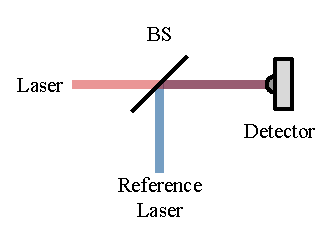
\includegraphics{part1/Figs/HeterodyneReferenceLaser.pdf}
    \end{subfigure}
    \begin{subfigure}{0.49\linewidth}
    %\centering
    %% Creator: Matplotlib, PGF backend
%%
%% To include the figure in your LaTeX document, write
%%   \input{<filename>.pgf}
%%
%% Make sure the required packages are loaded in your preamble
%%   \usepackage{pgf}
%%
%% Figures using additional raster images can only be included by \input if
%% they are in the same directory as the main LaTeX file. For loading figures
%% from other directories you can use the `import` package
%%   \usepackage{import}
%% and then include the figures with
%%   \import{<path to file>}{<filename>.pgf}
%%
%% Matplotlib used the following preamble
%%
\begingroup%
\makeatletter%
\begin{pgfpicture}%
\pgfpathrectangle{\pgfpointorigin}{\pgfqpoint{2.855000in}{1.427500in}}%
\pgfusepath{use as bounding box, clip}%
\begin{pgfscope}%
\pgfsetbuttcap%
\pgfsetmiterjoin%
\definecolor{currentfill}{rgb}{1.000000,1.000000,1.000000}%
\pgfsetfillcolor{currentfill}%
\pgfsetlinewidth{0.000000pt}%
\definecolor{currentstroke}{rgb}{1.000000,1.000000,1.000000}%
\pgfsetstrokecolor{currentstroke}%
\pgfsetdash{}{0pt}%
\pgfpathmoveto{\pgfqpoint{0.000000in}{0.000000in}}%
\pgfpathlineto{\pgfqpoint{2.855000in}{0.000000in}}%
\pgfpathlineto{\pgfqpoint{2.855000in}{1.427500in}}%
\pgfpathlineto{\pgfqpoint{0.000000in}{1.427500in}}%
\pgfpathclose%
\pgfusepath{fill}%
\end{pgfscope}%
\begin{pgfscope}%
\pgfsetbuttcap%
\pgfsetmiterjoin%
\definecolor{currentfill}{rgb}{1.000000,1.000000,1.000000}%
\pgfsetfillcolor{currentfill}%
\pgfsetlinewidth{0.000000pt}%
\definecolor{currentstroke}{rgb}{0.000000,0.000000,0.000000}%
\pgfsetstrokecolor{currentstroke}%
\pgfsetstrokeopacity{0.000000}%
\pgfsetdash{}{0pt}%
\pgfpathmoveto{\pgfqpoint{0.342732in}{0.521851in}}%
\pgfpathlineto{\pgfqpoint{1.130154in}{0.521851in}}%
\pgfpathlineto{\pgfqpoint{1.130154in}{1.277500in}}%
\pgfpathlineto{\pgfqpoint{0.342732in}{1.277500in}}%
\pgfpathclose%
\pgfusepath{fill}%
\end{pgfscope}%
\begin{pgfscope}%
\pgfpathrectangle{\pgfqpoint{0.342732in}{0.521851in}}{\pgfqpoint{0.787423in}{0.755649in}} %
\pgfusepath{clip}%
\pgfsetrectcap%
\pgfsetroundjoin%
\pgfsetlinewidth{1.003750pt}%
\definecolor{currentstroke}{rgb}{0.600000,0.000000,0.000000}%
\pgfsetstrokecolor{currentstroke}%
\pgfsetdash{}{0pt}%
\pgfpathmoveto{\pgfqpoint{0.342732in}{0.521851in}}%
\pgfpathlineto{\pgfqpoint{0.561854in}{0.522927in}}%
\pgfpathlineto{\pgfqpoint{0.578407in}{0.525366in}}%
\pgfpathlineto{\pgfqpoint{0.589442in}{0.529099in}}%
\pgfpathlineto{\pgfqpoint{0.598112in}{0.534189in}}%
\pgfpathlineto{\pgfqpoint{0.605994in}{0.541309in}}%
\pgfpathlineto{\pgfqpoint{0.613876in}{0.551728in}}%
\pgfpathlineto{\pgfqpoint{0.620970in}{0.564809in}}%
\pgfpathlineto{\pgfqpoint{0.628852in}{0.584548in}}%
\pgfpathlineto{\pgfqpoint{0.636734in}{0.610943in}}%
\pgfpathlineto{\pgfqpoint{0.644617in}{0.645114in}}%
\pgfpathlineto{\pgfqpoint{0.653287in}{0.692665in}}%
\pgfpathlineto{\pgfqpoint{0.663534in}{0.762770in}}%
\pgfpathlineto{\pgfqpoint{0.675357in}{0.860560in}}%
\pgfpathlineto{\pgfqpoint{0.715556in}{1.209829in}}%
\pgfpathlineto{\pgfqpoint{0.722649in}{1.247207in}}%
\pgfpathlineto{\pgfqpoint{0.728167in}{1.266451in}}%
\pgfpathlineto{\pgfqpoint{0.732896in}{1.275458in}}%
\pgfpathlineto{\pgfqpoint{0.736049in}{1.277475in}}%
\pgfpathlineto{\pgfqpoint{0.738414in}{1.276869in}}%
\pgfpathlineto{\pgfqpoint{0.741566in}{1.273247in}}%
\pgfpathlineto{\pgfqpoint{0.745508in}{1.264266in}}%
\pgfpathlineto{\pgfqpoint{0.750237in}{1.247207in}}%
\pgfpathlineto{\pgfqpoint{0.756542in}{1.214625in}}%
\pgfpathlineto{\pgfqpoint{0.764425in}{1.160406in}}%
\pgfpathlineto{\pgfqpoint{0.775460in}{1.066544in}}%
\pgfpathlineto{\pgfqpoint{0.810929in}{0.751028in}}%
\pgfpathlineto{\pgfqpoint{0.821964in}{0.678624in}}%
\pgfpathlineto{\pgfqpoint{0.831423in}{0.630451in}}%
\pgfpathlineto{\pgfqpoint{0.840093in}{0.596839in}}%
\pgfpathlineto{\pgfqpoint{0.848763in}{0.571983in}}%
\pgfpathlineto{\pgfqpoint{0.856645in}{0.555654in}}%
\pgfpathlineto{\pgfqpoint{0.864527in}{0.544042in}}%
\pgfpathlineto{\pgfqpoint{0.872410in}{0.536036in}}%
\pgfpathlineto{\pgfqpoint{0.881080in}{0.530257in}}%
\pgfpathlineto{\pgfqpoint{0.891327in}{0.526196in}}%
\pgfpathlineto{\pgfqpoint{0.903938in}{0.523664in}}%
\pgfpathlineto{\pgfqpoint{0.923643in}{0.522255in}}%
\pgfpathlineto{\pgfqpoint{0.970936in}{0.521857in}}%
\pgfpathlineto{\pgfqpoint{1.130154in}{0.521851in}}%
\pgfpathlineto{\pgfqpoint{1.130154in}{0.521851in}}%
\pgfusepath{stroke}%
\end{pgfscope}%
\begin{pgfscope}%
\pgfsetrectcap%
\pgfsetmiterjoin%
\pgfsetlinewidth{1.003750pt}%
\definecolor{currentstroke}{rgb}{0.000000,0.000000,0.000000}%
\pgfsetstrokecolor{currentstroke}%
\pgfsetdash{}{0pt}%
\pgfpathmoveto{\pgfqpoint{1.130154in}{0.521851in}}%
\pgfpathlineto{\pgfqpoint{1.130154in}{1.277500in}}%
\pgfusepath{stroke}%
\end{pgfscope}%
\begin{pgfscope}%
\pgfsetrectcap%
\pgfsetmiterjoin%
\pgfsetlinewidth{1.003750pt}%
\definecolor{currentstroke}{rgb}{0.000000,0.000000,0.000000}%
\pgfsetstrokecolor{currentstroke}%
\pgfsetdash{}{0pt}%
\pgfpathmoveto{\pgfqpoint{0.342732in}{1.277500in}}%
\pgfpathlineto{\pgfqpoint{1.130154in}{1.277500in}}%
\pgfusepath{stroke}%
\end{pgfscope}%
\begin{pgfscope}%
\pgfsetrectcap%
\pgfsetmiterjoin%
\pgfsetlinewidth{1.003750pt}%
\definecolor{currentstroke}{rgb}{0.000000,0.000000,0.000000}%
\pgfsetstrokecolor{currentstroke}%
\pgfsetdash{}{0pt}%
\pgfpathmoveto{\pgfqpoint{0.342732in}{0.521851in}}%
\pgfpathlineto{\pgfqpoint{1.130154in}{0.521851in}}%
\pgfusepath{stroke}%
\end{pgfscope}%
\begin{pgfscope}%
\pgfsetrectcap%
\pgfsetmiterjoin%
\pgfsetlinewidth{1.003750pt}%
\definecolor{currentstroke}{rgb}{0.000000,0.000000,0.000000}%
\pgfsetstrokecolor{currentstroke}%
\pgfsetdash{}{0pt}%
\pgfpathmoveto{\pgfqpoint{0.342732in}{0.521851in}}%
\pgfpathlineto{\pgfqpoint{0.342732in}{1.277500in}}%
\pgfusepath{stroke}%
\end{pgfscope}%
\begin{pgfscope}%
\pgfsetbuttcap%
\pgfsetroundjoin%
\definecolor{currentfill}{rgb}{0.000000,0.000000,0.000000}%
\pgfsetfillcolor{currentfill}%
\pgfsetlinewidth{0.501875pt}%
\definecolor{currentstroke}{rgb}{0.000000,0.000000,0.000000}%
\pgfsetstrokecolor{currentstroke}%
\pgfsetdash{}{0pt}%
\pgfsys@defobject{currentmarker}{\pgfqpoint{0.000000in}{0.000000in}}{\pgfqpoint{0.000000in}{0.055556in}}{%
\pgfpathmoveto{\pgfqpoint{0.000000in}{0.000000in}}%
\pgfpathlineto{\pgfqpoint{0.000000in}{0.055556in}}%
\pgfusepath{stroke,fill}%
}%
\begin{pgfscope}%
\pgfsys@transformshift{0.736443in}{0.521851in}%
\pgfsys@useobject{currentmarker}{}%
\end{pgfscope}%
\end{pgfscope}%
\begin{pgfscope}%
\pgfsetbuttcap%
\pgfsetroundjoin%
\definecolor{currentfill}{rgb}{0.000000,0.000000,0.000000}%
\pgfsetfillcolor{currentfill}%
\pgfsetlinewidth{0.501875pt}%
\definecolor{currentstroke}{rgb}{0.000000,0.000000,0.000000}%
\pgfsetstrokecolor{currentstroke}%
\pgfsetdash{}{0pt}%
\pgfsys@defobject{currentmarker}{\pgfqpoint{0.000000in}{-0.055556in}}{\pgfqpoint{0.000000in}{0.000000in}}{%
\pgfpathmoveto{\pgfqpoint{0.000000in}{0.000000in}}%
\pgfpathlineto{\pgfqpoint{0.000000in}{-0.055556in}}%
\pgfusepath{stroke,fill}%
}%
\begin{pgfscope}%
\pgfsys@transformshift{0.736443in}{1.277500in}%
\pgfsys@useobject{currentmarker}{}%
\end{pgfscope}%
\end{pgfscope}%
\begin{pgfscope}%
\pgftext[x=0.736443in,y=0.466296in,,top]{\fontsize{10.000000}{12.000000}\selectfont \(\displaystyle \omega_1\)}%
\end{pgfscope}%
\begin{pgfscope}%
\pgftext[x=0.273287in,y=0.899676in,,bottom,rotate=90.000000]{\fontsize{10.000000}{12.000000}\selectfont Amplitude}%
\end{pgfscope}%
\begin{pgfscope}%
\pgfsetbuttcap%
\pgfsetmiterjoin%
\definecolor{currentfill}{rgb}{1.000000,1.000000,1.000000}%
\pgfsetfillcolor{currentfill}%
\pgfsetlinewidth{0.000000pt}%
\definecolor{currentstroke}{rgb}{0.000000,0.000000,0.000000}%
\pgfsetstrokecolor{currentstroke}%
\pgfsetstrokeopacity{0.000000}%
\pgfsetdash{}{0pt}%
\pgfpathmoveto{\pgfqpoint{1.130154in}{0.521851in}}%
\pgfpathlineto{\pgfqpoint{1.917577in}{0.521851in}}%
\pgfpathlineto{\pgfqpoint{1.917577in}{1.277500in}}%
\pgfpathlineto{\pgfqpoint{1.130154in}{1.277500in}}%
\pgfpathclose%
\pgfusepath{fill}%
\end{pgfscope}%
\begin{pgfscope}%
\pgfpathrectangle{\pgfqpoint{1.130154in}{0.521851in}}{\pgfqpoint{0.787423in}{0.755649in}} %
\pgfusepath{clip}%
\pgfsetrectcap%
\pgfsetroundjoin%
\pgfsetlinewidth{1.003750pt}%
\definecolor{currentstroke}{rgb}{0.043137,0.325490,0.580392}%
\pgfsetstrokecolor{currentstroke}%
\pgfsetdash{}{0pt}%
\pgfpathmoveto{\pgfqpoint{1.130154in}{0.521851in}}%
\pgfpathlineto{\pgfqpoint{1.491943in}{0.522906in}}%
\pgfpathlineto{\pgfqpoint{1.495096in}{0.525477in}}%
\pgfpathlineto{\pgfqpoint{1.497461in}{0.530263in}}%
\pgfpathlineto{\pgfqpoint{1.499825in}{0.540010in}}%
\pgfpathlineto{\pgfqpoint{1.502190in}{0.558322in}}%
\pgfpathlineto{\pgfqpoint{1.505343in}{0.604463in}}%
\pgfpathlineto{\pgfqpoint{1.508496in}{0.686453in}}%
\pgfpathlineto{\pgfqpoint{1.513225in}{0.885838in}}%
\pgfpathlineto{\pgfqpoint{1.521107in}{1.241295in}}%
\pgfpathlineto{\pgfqpoint{1.523472in}{1.276743in}}%
\pgfpathlineto{\pgfqpoint{1.524260in}{1.276743in}}%
\pgfpathlineto{\pgfqpoint{1.525836in}{1.258806in}}%
\pgfpathlineto{\pgfqpoint{1.528201in}{1.191219in}}%
\pgfpathlineto{\pgfqpoint{1.532930in}{0.966603in}}%
\pgfpathlineto{\pgfqpoint{1.539236in}{0.686453in}}%
\pgfpathlineto{\pgfqpoint{1.543177in}{0.590005in}}%
\pgfpathlineto{\pgfqpoint{1.547118in}{0.544946in}}%
\pgfpathlineto{\pgfqpoint{1.550271in}{0.530263in}}%
\pgfpathlineto{\pgfqpoint{1.553424in}{0.524546in}}%
\pgfpathlineto{\pgfqpoint{1.557365in}{0.522394in}}%
\pgfpathlineto{\pgfqpoint{1.565247in}{0.521863in}}%
\pgfpathlineto{\pgfqpoint{1.777276in}{0.521851in}}%
\pgfpathlineto{\pgfqpoint{1.917577in}{0.521851in}}%
\pgfpathlineto{\pgfqpoint{1.917577in}{0.521851in}}%
\pgfusepath{stroke}%
\end{pgfscope}%
\begin{pgfscope}%
\pgfsetrectcap%
\pgfsetmiterjoin%
\pgfsetlinewidth{1.003750pt}%
\definecolor{currentstroke}{rgb}{0.000000,0.000000,0.000000}%
\pgfsetstrokecolor{currentstroke}%
\pgfsetdash{}{0pt}%
\pgfpathmoveto{\pgfqpoint{1.917577in}{0.521851in}}%
\pgfpathlineto{\pgfqpoint{1.917577in}{1.277500in}}%
\pgfusepath{stroke}%
\end{pgfscope}%
\begin{pgfscope}%
\pgfsetrectcap%
\pgfsetmiterjoin%
\pgfsetlinewidth{1.003750pt}%
\definecolor{currentstroke}{rgb}{0.000000,0.000000,0.000000}%
\pgfsetstrokecolor{currentstroke}%
\pgfsetdash{}{0pt}%
\pgfpathmoveto{\pgfqpoint{1.130154in}{1.277500in}}%
\pgfpathlineto{\pgfqpoint{1.917577in}{1.277500in}}%
\pgfusepath{stroke}%
\end{pgfscope}%
\begin{pgfscope}%
\pgfsetrectcap%
\pgfsetmiterjoin%
\pgfsetlinewidth{1.003750pt}%
\definecolor{currentstroke}{rgb}{0.000000,0.000000,0.000000}%
\pgfsetstrokecolor{currentstroke}%
\pgfsetdash{}{0pt}%
\pgfpathmoveto{\pgfqpoint{1.130154in}{0.521851in}}%
\pgfpathlineto{\pgfqpoint{1.917577in}{0.521851in}}%
\pgfusepath{stroke}%
\end{pgfscope}%
\begin{pgfscope}%
\pgfsetrectcap%
\pgfsetmiterjoin%
\pgfsetlinewidth{1.003750pt}%
\definecolor{currentstroke}{rgb}{0.000000,0.000000,0.000000}%
\pgfsetstrokecolor{currentstroke}%
\pgfsetdash{}{0pt}%
\pgfpathmoveto{\pgfqpoint{1.130154in}{0.521851in}}%
\pgfpathlineto{\pgfqpoint{1.130154in}{1.277500in}}%
\pgfusepath{stroke}%
\end{pgfscope}%
\begin{pgfscope}%
\pgfsetbuttcap%
\pgfsetroundjoin%
\definecolor{currentfill}{rgb}{0.000000,0.000000,0.000000}%
\pgfsetfillcolor{currentfill}%
\pgfsetlinewidth{0.501875pt}%
\definecolor{currentstroke}{rgb}{0.000000,0.000000,0.000000}%
\pgfsetstrokecolor{currentstroke}%
\pgfsetdash{}{0pt}%
\pgfsys@defobject{currentmarker}{\pgfqpoint{0.000000in}{0.000000in}}{\pgfqpoint{0.000000in}{0.055556in}}{%
\pgfpathmoveto{\pgfqpoint{0.000000in}{0.000000in}}%
\pgfpathlineto{\pgfqpoint{0.000000in}{0.055556in}}%
\pgfusepath{stroke,fill}%
}%
\begin{pgfscope}%
\pgfsys@transformshift{1.523866in}{0.521851in}%
\pgfsys@useobject{currentmarker}{}%
\end{pgfscope}%
\end{pgfscope}%
\begin{pgfscope}%
\pgfsetbuttcap%
\pgfsetroundjoin%
\definecolor{currentfill}{rgb}{0.000000,0.000000,0.000000}%
\pgfsetfillcolor{currentfill}%
\pgfsetlinewidth{0.501875pt}%
\definecolor{currentstroke}{rgb}{0.000000,0.000000,0.000000}%
\pgfsetstrokecolor{currentstroke}%
\pgfsetdash{}{0pt}%
\pgfsys@defobject{currentmarker}{\pgfqpoint{0.000000in}{-0.055556in}}{\pgfqpoint{0.000000in}{0.000000in}}{%
\pgfpathmoveto{\pgfqpoint{0.000000in}{0.000000in}}%
\pgfpathlineto{\pgfqpoint{0.000000in}{-0.055556in}}%
\pgfusepath{stroke,fill}%
}%
\begin{pgfscope}%
\pgfsys@transformshift{1.523866in}{1.277500in}%
\pgfsys@useobject{currentmarker}{}%
\end{pgfscope}%
\end{pgfscope}%
\begin{pgfscope}%
\pgftext[x=1.523866in,y=0.466296in,,top]{\fontsize{10.000000}{12.000000}\selectfont \(\displaystyle \omega_2\)}%
\end{pgfscope}%
\begin{pgfscope}%
\pgftext[x=1.523866in,y=0.273395in,,top]{\fontsize{10.000000}{12.000000}\selectfont Frequency}%
\end{pgfscope}%
\begin{pgfscope}%
\pgfsetbuttcap%
\pgfsetmiterjoin%
\definecolor{currentfill}{rgb}{1.000000,1.000000,1.000000}%
\pgfsetfillcolor{currentfill}%
\pgfsetlinewidth{0.000000pt}%
\definecolor{currentstroke}{rgb}{0.000000,0.000000,0.000000}%
\pgfsetstrokecolor{currentstroke}%
\pgfsetstrokeopacity{0.000000}%
\pgfsetdash{}{0pt}%
\pgfpathmoveto{\pgfqpoint{1.917577in}{0.521851in}}%
\pgfpathlineto{\pgfqpoint{2.705000in}{0.521851in}}%
\pgfpathlineto{\pgfqpoint{2.705000in}{1.277500in}}%
\pgfpathlineto{\pgfqpoint{1.917577in}{1.277500in}}%
\pgfpathclose%
\pgfusepath{fill}%
\end{pgfscope}%
\begin{pgfscope}%
\pgfpathrectangle{\pgfqpoint{1.917577in}{0.521851in}}{\pgfqpoint{0.787423in}{0.755649in}} %
\pgfusepath{clip}%
\pgfsetrectcap%
\pgfsetroundjoin%
\pgfsetlinewidth{1.003750pt}%
\definecolor{currentstroke}{rgb}{0.301961,0.607843,0.301961}%
\pgfsetstrokecolor{currentstroke}%
\pgfsetdash{}{0pt}%
\pgfpathmoveto{\pgfqpoint{1.917577in}{0.521851in}}%
\pgfpathlineto{\pgfqpoint{2.134335in}{0.522937in}}%
\pgfpathlineto{\pgfqpoint{2.150888in}{0.525331in}}%
\pgfpathlineto{\pgfqpoint{2.161923in}{0.528952in}}%
\pgfpathlineto{\pgfqpoint{2.171381in}{0.534419in}}%
\pgfpathlineto{\pgfqpoint{2.179263in}{0.541509in}}%
\pgfpathlineto{\pgfqpoint{2.187145in}{0.551814in}}%
\pgfpathlineto{\pgfqpoint{2.194239in}{0.564679in}}%
\pgfpathlineto{\pgfqpoint{2.202121in}{0.584001in}}%
\pgfpathlineto{\pgfqpoint{2.210004in}{0.609738in}}%
\pgfpathlineto{\pgfqpoint{2.218674in}{0.646729in}}%
\pgfpathlineto{\pgfqpoint{2.227344in}{0.693823in}}%
\pgfpathlineto{\pgfqpoint{2.237591in}{0.762940in}}%
\pgfpathlineto{\pgfqpoint{2.249414in}{0.859050in}}%
\pgfpathlineto{\pgfqpoint{2.290401in}{1.209531in}}%
\pgfpathlineto{\pgfqpoint{2.297495in}{1.246500in}}%
\pgfpathlineto{\pgfqpoint{2.303012in}{1.265770in}}%
\pgfpathlineto{\pgfqpoint{2.307742in}{1.275061in}}%
\pgfpathlineto{\pgfqpoint{2.310895in}{1.277402in}}%
\pgfpathlineto{\pgfqpoint{2.313259in}{1.277109in}}%
\pgfpathlineto{\pgfqpoint{2.316412in}{1.273991in}}%
\pgfpathlineto{\pgfqpoint{2.320353in}{1.265770in}}%
\pgfpathlineto{\pgfqpoint{2.325082in}{1.249786in}}%
\pgfpathlineto{\pgfqpoint{2.331388in}{1.218840in}}%
\pgfpathlineto{\pgfqpoint{2.339270in}{1.166816in}}%
\pgfpathlineto{\pgfqpoint{2.349517in}{1.082834in}}%
\pgfpathlineto{\pgfqpoint{2.389716in}{0.734661in}}%
\pgfpathlineto{\pgfqpoint{2.399962in}{0.671121in}}%
\pgfpathlineto{\pgfqpoint{2.409421in}{0.625355in}}%
\pgfpathlineto{\pgfqpoint{2.418091in}{0.593463in}}%
\pgfpathlineto{\pgfqpoint{2.426762in}{0.569871in}}%
\pgfpathlineto{\pgfqpoint{2.434644in}{0.554349in}}%
\pgfpathlineto{\pgfqpoint{2.442526in}{0.543282in}}%
\pgfpathlineto{\pgfqpoint{2.451196in}{0.535009in}}%
\pgfpathlineto{\pgfqpoint{2.460655in}{0.529309in}}%
\pgfpathlineto{\pgfqpoint{2.471690in}{0.525519in}}%
\pgfpathlineto{\pgfqpoint{2.485877in}{0.523219in}}%
\pgfpathlineto{\pgfqpoint{2.508735in}{0.522085in}}%
\pgfpathlineto{\pgfqpoint{2.580463in}{0.521852in}}%
\pgfpathlineto{\pgfqpoint{2.705000in}{0.521851in}}%
\pgfpathlineto{\pgfqpoint{2.705000in}{0.521851in}}%
\pgfusepath{stroke}%
\end{pgfscope}%
\begin{pgfscope}%
\pgfpathrectangle{\pgfqpoint{1.917577in}{0.521851in}}{\pgfqpoint{0.787423in}{0.755649in}} %
\pgfusepath{clip}%
\pgfsetbuttcap%
\pgfsetroundjoin%
\pgfsetlinewidth{1.003750pt}%
\definecolor{currentstroke}{rgb}{0.043137,0.325490,0.580392}%
\pgfsetstrokecolor{currentstroke}%
\pgfsetdash{{1.000000pt}{3.000000pt}}{0.000000pt}%
\pgfpathmoveto{\pgfqpoint{1.917577in}{0.521851in}}%
\pgfpathlineto{\pgfqpoint{2.279366in}{0.522906in}}%
\pgfpathlineto{\pgfqpoint{2.282519in}{0.525477in}}%
\pgfpathlineto{\pgfqpoint{2.284884in}{0.530263in}}%
\pgfpathlineto{\pgfqpoint{2.287248in}{0.540010in}}%
\pgfpathlineto{\pgfqpoint{2.289613in}{0.558322in}}%
\pgfpathlineto{\pgfqpoint{2.292766in}{0.604463in}}%
\pgfpathlineto{\pgfqpoint{2.295919in}{0.686453in}}%
\pgfpathlineto{\pgfqpoint{2.300648in}{0.885838in}}%
\pgfpathlineto{\pgfqpoint{2.308530in}{1.241295in}}%
\pgfpathlineto{\pgfqpoint{2.310895in}{1.276743in}}%
\pgfpathlineto{\pgfqpoint{2.311683in}{1.276743in}}%
\pgfpathlineto{\pgfqpoint{2.313259in}{1.258806in}}%
\pgfpathlineto{\pgfqpoint{2.315624in}{1.191219in}}%
\pgfpathlineto{\pgfqpoint{2.320353in}{0.966603in}}%
\pgfpathlineto{\pgfqpoint{2.326659in}{0.686453in}}%
\pgfpathlineto{\pgfqpoint{2.330600in}{0.590005in}}%
\pgfpathlineto{\pgfqpoint{2.334541in}{0.544946in}}%
\pgfpathlineto{\pgfqpoint{2.337694in}{0.530263in}}%
\pgfpathlineto{\pgfqpoint{2.340847in}{0.524546in}}%
\pgfpathlineto{\pgfqpoint{2.344788in}{0.522394in}}%
\pgfpathlineto{\pgfqpoint{2.352670in}{0.521863in}}%
\pgfpathlineto{\pgfqpoint{2.564698in}{0.521851in}}%
\pgfpathlineto{\pgfqpoint{2.705000in}{0.521851in}}%
\pgfpathlineto{\pgfqpoint{2.705000in}{0.521851in}}%
\pgfusepath{stroke}%
\end{pgfscope}%
\begin{pgfscope}%
\pgfpathrectangle{\pgfqpoint{1.917577in}{0.521851in}}{\pgfqpoint{0.787423in}{0.755649in}} %
\pgfusepath{clip}%
\pgfsetbuttcap%
\pgfsetroundjoin%
\pgfsetlinewidth{1.003750pt}%
\definecolor{currentstroke}{rgb}{0.600000,0.000000,0.000000}%
\pgfsetstrokecolor{currentstroke}%
\pgfsetdash{{1.000000pt}{3.000000pt}}{0.000000pt}%
\pgfpathmoveto{\pgfqpoint{1.917577in}{0.521851in}}%
\pgfpathlineto{\pgfqpoint{2.136700in}{0.522927in}}%
\pgfpathlineto{\pgfqpoint{2.153252in}{0.525366in}}%
\pgfpathlineto{\pgfqpoint{2.164287in}{0.529099in}}%
\pgfpathlineto{\pgfqpoint{2.172958in}{0.534189in}}%
\pgfpathlineto{\pgfqpoint{2.180840in}{0.541309in}}%
\pgfpathlineto{\pgfqpoint{2.188722in}{0.551728in}}%
\pgfpathlineto{\pgfqpoint{2.195816in}{0.564809in}}%
\pgfpathlineto{\pgfqpoint{2.203698in}{0.584548in}}%
\pgfpathlineto{\pgfqpoint{2.211580in}{0.610943in}}%
\pgfpathlineto{\pgfqpoint{2.219462in}{0.645114in}}%
\pgfpathlineto{\pgfqpoint{2.228132in}{0.692665in}}%
\pgfpathlineto{\pgfqpoint{2.238379in}{0.762770in}}%
\pgfpathlineto{\pgfqpoint{2.250202in}{0.860560in}}%
\pgfpathlineto{\pgfqpoint{2.290401in}{1.209829in}}%
\pgfpathlineto{\pgfqpoint{2.297495in}{1.247207in}}%
\pgfpathlineto{\pgfqpoint{2.303012in}{1.266451in}}%
\pgfpathlineto{\pgfqpoint{2.307742in}{1.275458in}}%
\pgfpathlineto{\pgfqpoint{2.310895in}{1.277475in}}%
\pgfpathlineto{\pgfqpoint{2.313259in}{1.276869in}}%
\pgfpathlineto{\pgfqpoint{2.316412in}{1.273247in}}%
\pgfpathlineto{\pgfqpoint{2.320353in}{1.264266in}}%
\pgfpathlineto{\pgfqpoint{2.325082in}{1.247207in}}%
\pgfpathlineto{\pgfqpoint{2.331388in}{1.214625in}}%
\pgfpathlineto{\pgfqpoint{2.339270in}{1.160406in}}%
\pgfpathlineto{\pgfqpoint{2.350305in}{1.066544in}}%
\pgfpathlineto{\pgfqpoint{2.385775in}{0.751028in}}%
\pgfpathlineto{\pgfqpoint{2.396810in}{0.678624in}}%
\pgfpathlineto{\pgfqpoint{2.406268in}{0.630451in}}%
\pgfpathlineto{\pgfqpoint{2.414938in}{0.596839in}}%
\pgfpathlineto{\pgfqpoint{2.423609in}{0.571983in}}%
\pgfpathlineto{\pgfqpoint{2.431491in}{0.555654in}}%
\pgfpathlineto{\pgfqpoint{2.439373in}{0.544042in}}%
\pgfpathlineto{\pgfqpoint{2.447255in}{0.536036in}}%
\pgfpathlineto{\pgfqpoint{2.455925in}{0.530257in}}%
\pgfpathlineto{\pgfqpoint{2.466172in}{0.526196in}}%
\pgfpathlineto{\pgfqpoint{2.478783in}{0.523664in}}%
\pgfpathlineto{\pgfqpoint{2.498489in}{0.522255in}}%
\pgfpathlineto{\pgfqpoint{2.545781in}{0.521857in}}%
\pgfpathlineto{\pgfqpoint{2.705000in}{0.521851in}}%
\pgfpathlineto{\pgfqpoint{2.705000in}{0.521851in}}%
\pgfusepath{stroke}%
\end{pgfscope}%
\begin{pgfscope}%
\pgfsetrectcap%
\pgfsetmiterjoin%
\pgfsetlinewidth{1.003750pt}%
\definecolor{currentstroke}{rgb}{0.000000,0.000000,0.000000}%
\pgfsetstrokecolor{currentstroke}%
\pgfsetdash{}{0pt}%
\pgfpathmoveto{\pgfqpoint{2.705000in}{0.521851in}}%
\pgfpathlineto{\pgfqpoint{2.705000in}{1.277500in}}%
\pgfusepath{stroke}%
\end{pgfscope}%
\begin{pgfscope}%
\pgfsetrectcap%
\pgfsetmiterjoin%
\pgfsetlinewidth{1.003750pt}%
\definecolor{currentstroke}{rgb}{0.000000,0.000000,0.000000}%
\pgfsetstrokecolor{currentstroke}%
\pgfsetdash{}{0pt}%
\pgfpathmoveto{\pgfqpoint{1.917577in}{1.277500in}}%
\pgfpathlineto{\pgfqpoint{2.705000in}{1.277500in}}%
\pgfusepath{stroke}%
\end{pgfscope}%
\begin{pgfscope}%
\pgfsetrectcap%
\pgfsetmiterjoin%
\pgfsetlinewidth{1.003750pt}%
\definecolor{currentstroke}{rgb}{0.000000,0.000000,0.000000}%
\pgfsetstrokecolor{currentstroke}%
\pgfsetdash{}{0pt}%
\pgfpathmoveto{\pgfqpoint{1.917577in}{0.521851in}}%
\pgfpathlineto{\pgfqpoint{2.705000in}{0.521851in}}%
\pgfusepath{stroke}%
\end{pgfscope}%
\begin{pgfscope}%
\pgfsetrectcap%
\pgfsetmiterjoin%
\pgfsetlinewidth{1.003750pt}%
\definecolor{currentstroke}{rgb}{0.000000,0.000000,0.000000}%
\pgfsetstrokecolor{currentstroke}%
\pgfsetdash{}{0pt}%
\pgfpathmoveto{\pgfqpoint{1.917577in}{0.521851in}}%
\pgfpathlineto{\pgfqpoint{1.917577in}{1.277500in}}%
\pgfusepath{stroke}%
\end{pgfscope}%
\begin{pgfscope}%
\pgfsetbuttcap%
\pgfsetroundjoin%
\definecolor{currentfill}{rgb}{0.000000,0.000000,0.000000}%
\pgfsetfillcolor{currentfill}%
\pgfsetlinewidth{0.501875pt}%
\definecolor{currentstroke}{rgb}{0.000000,0.000000,0.000000}%
\pgfsetstrokecolor{currentstroke}%
\pgfsetdash{}{0pt}%
\pgfsys@defobject{currentmarker}{\pgfqpoint{0.000000in}{0.000000in}}{\pgfqpoint{0.000000in}{0.055556in}}{%
\pgfpathmoveto{\pgfqpoint{0.000000in}{0.000000in}}%
\pgfpathlineto{\pgfqpoint{0.000000in}{0.055556in}}%
\pgfusepath{stroke,fill}%
}%
\begin{pgfscope}%
\pgfsys@transformshift{2.311289in}{0.521851in}%
\pgfsys@useobject{currentmarker}{}%
\end{pgfscope}%
\end{pgfscope}%
\begin{pgfscope}%
\pgfsetbuttcap%
\pgfsetroundjoin%
\definecolor{currentfill}{rgb}{0.000000,0.000000,0.000000}%
\pgfsetfillcolor{currentfill}%
\pgfsetlinewidth{0.501875pt}%
\definecolor{currentstroke}{rgb}{0.000000,0.000000,0.000000}%
\pgfsetstrokecolor{currentstroke}%
\pgfsetdash{}{0pt}%
\pgfsys@defobject{currentmarker}{\pgfqpoint{0.000000in}{-0.055556in}}{\pgfqpoint{0.000000in}{0.000000in}}{%
\pgfpathmoveto{\pgfqpoint{0.000000in}{0.000000in}}%
\pgfpathlineto{\pgfqpoint{0.000000in}{-0.055556in}}%
\pgfusepath{stroke,fill}%
}%
\begin{pgfscope}%
\pgfsys@transformshift{2.311289in}{1.277500in}%
\pgfsys@useobject{currentmarker}{}%
\end{pgfscope}%
\end{pgfscope}%
\begin{pgfscope}%
\pgftext[x=2.311289in,y=0.466296in,,top]{\fontsize{10.000000}{12.000000}\selectfont \(\displaystyle \omega_1-\omega_2\)}%
\end{pgfscope}%
\end{pgfpicture}%
\makeatother%
\endgroup%

    \end{subfigure}
    \caption{Heterodyne measurement with a narrow reference laser by combining the laser of interest ($\omega_1$, red) with the reference laser ($\omega_2$, blue). Shown on the right is the spectral lineshapes of the lasers and the heterodyne beatnote (green).}
    \label{figure:heterodyne_reference}
\end{figure}

The initial intention with the experiments described in the this chapter was to be able to use a \gls{pdh} locked laser as a frequency reference to characterise the performance of another laser locked with \gls{ps} using high-bandwidth feedback.
Unfortunately, initial measurements were unable to confirm that the \gls{pdh} locked laser was in fact much narrower than \gls{ps} locked one so more sophisticated methods were required.

\subsubsection{Self-heterodyne}

The self-heterodyne technique involves beating a laser with itself in order to perform a heterodyne measurement, as shown in Figure~\ref{figure:heterodyne_reference}~\cite{okoshi_novel_1980}.
In order to perform this measurement it is necessary to split the laser into two beams and frequency shift on beam, usually with an \gls{aom}, such that the beatnote is not centred at \unit[0]{Hz}.
The two beams are still correlated so it is necessary to propagate one beam to reduce the coherence otherwise the lineshape of the beatnote would just appear as a delta function centred at the \gls{aom} frequency~\cite{richter_linewidth_1986}.
One beam of the beams is typically delayed by a very long optical fibre such that that arm of the heterodyne measurement has been delayed, ideally for as long as the coherence time of the laser.
Practically this would require optical fibres with lengths from 1 to \unit[100]{km} depending on the linewidth of the laser under investigation.
Unfortunately the absorption losses in fibres tends to be at least a few dB per kilometre making fibres longer than \unit[10]{km} troublesome to use.

\begin{figure}
    %\centering
    \begin{subfigure}{0.49\linewidth}
    %\centering
    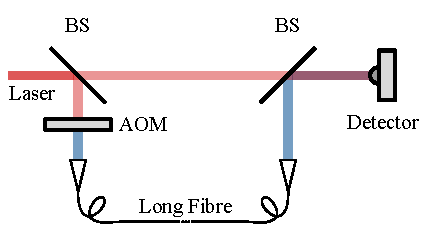
\includegraphics{part1/Figs/SelfHeterodyne.pdf}
    \end{subfigure}
    \begin{subfigure}{0.49\linewidth}
    %\centering
    %% Creator: Matplotlib, PGF backend
%%
%% To include the figure in your LaTeX document, write
%%   \input{<filename>.pgf}
%%
%% Make sure the required packages are loaded in your preamble
%%   \usepackage{pgf}
%%
%% Figures using additional raster images can only be included by \input if
%% they are in the same directory as the main LaTeX file. For loading figures
%% from other directories you can use the `import` package
%%   \usepackage{import}
%% and then include the figures with
%%   \import{<path to file>}{<filename>.pgf}
%%
%% Matplotlib used the following preamble
%%
\begingroup%
\makeatletter%
\begin{pgfpicture}%
\pgfpathrectangle{\pgfpointorigin}{\pgfqpoint{2.855000in}{1.427500in}}%
\pgfusepath{use as bounding box, clip}%
\begin{pgfscope}%
\pgfsetbuttcap%
\pgfsetmiterjoin%
\definecolor{currentfill}{rgb}{1.000000,1.000000,1.000000}%
\pgfsetfillcolor{currentfill}%
\pgfsetlinewidth{0.000000pt}%
\definecolor{currentstroke}{rgb}{1.000000,1.000000,1.000000}%
\pgfsetstrokecolor{currentstroke}%
\pgfsetdash{}{0pt}%
\pgfpathmoveto{\pgfqpoint{0.000000in}{0.000000in}}%
\pgfpathlineto{\pgfqpoint{2.855000in}{0.000000in}}%
\pgfpathlineto{\pgfqpoint{2.855000in}{1.427500in}}%
\pgfpathlineto{\pgfqpoint{0.000000in}{1.427500in}}%
\pgfpathclose%
\pgfusepath{fill}%
\end{pgfscope}%
\begin{pgfscope}%
\pgfsetbuttcap%
\pgfsetmiterjoin%
\definecolor{currentfill}{rgb}{1.000000,1.000000,1.000000}%
\pgfsetfillcolor{currentfill}%
\pgfsetlinewidth{0.000000pt}%
\definecolor{currentstroke}{rgb}{0.000000,0.000000,0.000000}%
\pgfsetstrokecolor{currentstroke}%
\pgfsetstrokeopacity{0.000000}%
\pgfsetdash{}{0pt}%
\pgfpathmoveto{\pgfqpoint{0.342732in}{0.521851in}}%
\pgfpathlineto{\pgfqpoint{1.130154in}{0.521851in}}%
\pgfpathlineto{\pgfqpoint{1.130154in}{1.277500in}}%
\pgfpathlineto{\pgfqpoint{0.342732in}{1.277500in}}%
\pgfpathclose%
\pgfusepath{fill}%
\end{pgfscope}%
\begin{pgfscope}%
\pgfpathrectangle{\pgfqpoint{0.342732in}{0.521851in}}{\pgfqpoint{0.787423in}{0.755649in}} %
\pgfusepath{clip}%
\pgfsetrectcap%
\pgfsetroundjoin%
\pgfsetlinewidth{1.003750pt}%
\definecolor{currentstroke}{rgb}{0.600000,0.000000,0.000000}%
\pgfsetstrokecolor{currentstroke}%
\pgfsetdash{}{0pt}%
\pgfpathmoveto{\pgfqpoint{0.342732in}{0.521851in}}%
\pgfpathlineto{\pgfqpoint{0.564219in}{0.522921in}}%
\pgfpathlineto{\pgfqpoint{0.580771in}{0.525286in}}%
\pgfpathlineto{\pgfqpoint{0.592595in}{0.529207in}}%
\pgfpathlineto{\pgfqpoint{0.602053in}{0.534806in}}%
\pgfpathlineto{\pgfqpoint{0.609935in}{0.542011in}}%
\pgfpathlineto{\pgfqpoint{0.617817in}{0.552396in}}%
\pgfpathlineto{\pgfqpoint{0.625699in}{0.566909in}}%
\pgfpathlineto{\pgfqpoint{0.633582in}{0.586567in}}%
\pgfpathlineto{\pgfqpoint{0.641464in}{0.612351in}}%
\pgfpathlineto{\pgfqpoint{0.650134in}{0.648745in}}%
\pgfpathlineto{\pgfqpoint{0.659593in}{0.698686in}}%
\pgfpathlineto{\pgfqpoint{0.670628in}{0.769933in}}%
\pgfpathlineto{\pgfqpoint{0.685604in}{0.883056in}}%
\pgfpathlineto{\pgfqpoint{0.707673in}{1.048886in}}%
\pgfpathlineto{\pgfqpoint{0.717132in}{1.103032in}}%
\pgfpathlineto{\pgfqpoint{0.724226in}{1.131667in}}%
\pgfpathlineto{\pgfqpoint{0.729743in}{1.145509in}}%
\pgfpathlineto{\pgfqpoint{0.733684in}{1.150529in}}%
\pgfpathlineto{\pgfqpoint{0.736837in}{1.151538in}}%
\pgfpathlineto{\pgfqpoint{0.739990in}{1.149857in}}%
\pgfpathlineto{\pgfqpoint{0.743143in}{1.145509in}}%
\pgfpathlineto{\pgfqpoint{0.747084in}{1.136411in}}%
\pgfpathlineto{\pgfqpoint{0.752601in}{1.117178in}}%
\pgfpathlineto{\pgfqpoint{0.759695in}{1.082441in}}%
\pgfpathlineto{\pgfqpoint{0.768366in}{1.027639in}}%
\pgfpathlineto{\pgfqpoint{0.781765in}{0.926710in}}%
\pgfpathlineto{\pgfqpoint{0.805412in}{0.748268in}}%
\pgfpathlineto{\pgfqpoint{0.817235in}{0.676571in}}%
\pgfpathlineto{\pgfqpoint{0.827481in}{0.627804in}}%
\pgfpathlineto{\pgfqpoint{0.836940in}{0.593618in}}%
\pgfpathlineto{\pgfqpoint{0.845610in}{0.570397in}}%
\pgfpathlineto{\pgfqpoint{0.854281in}{0.553645in}}%
\pgfpathlineto{\pgfqpoint{0.862163in}{0.542891in}}%
\pgfpathlineto{\pgfqpoint{0.870833in}{0.534806in}}%
\pgfpathlineto{\pgfqpoint{0.880292in}{0.529207in}}%
\pgfpathlineto{\pgfqpoint{0.891327in}{0.525472in}}%
\pgfpathlineto{\pgfqpoint{0.905514in}{0.523199in}}%
\pgfpathlineto{\pgfqpoint{0.928372in}{0.522080in}}%
\pgfpathlineto{\pgfqpoint{1.000888in}{0.521852in}}%
\pgfpathlineto{\pgfqpoint{1.130154in}{0.521851in}}%
\pgfpathlineto{\pgfqpoint{1.130154in}{0.521851in}}%
\pgfusepath{stroke}%
\end{pgfscope}%
\begin{pgfscope}%
\pgfsetrectcap%
\pgfsetmiterjoin%
\pgfsetlinewidth{1.003750pt}%
\definecolor{currentstroke}{rgb}{0.000000,0.000000,0.000000}%
\pgfsetstrokecolor{currentstroke}%
\pgfsetdash{}{0pt}%
\pgfpathmoveto{\pgfqpoint{0.342732in}{1.277500in}}%
\pgfpathlineto{\pgfqpoint{1.130154in}{1.277500in}}%
\pgfusepath{stroke}%
\end{pgfscope}%
\begin{pgfscope}%
\pgfsetrectcap%
\pgfsetmiterjoin%
\pgfsetlinewidth{1.003750pt}%
\definecolor{currentstroke}{rgb}{0.000000,0.000000,0.000000}%
\pgfsetstrokecolor{currentstroke}%
\pgfsetdash{}{0pt}%
\pgfpathmoveto{\pgfqpoint{0.342732in}{0.521851in}}%
\pgfpathlineto{\pgfqpoint{0.342732in}{1.277500in}}%
\pgfusepath{stroke}%
\end{pgfscope}%
\begin{pgfscope}%
\pgfsetrectcap%
\pgfsetmiterjoin%
\pgfsetlinewidth{1.003750pt}%
\definecolor{currentstroke}{rgb}{0.000000,0.000000,0.000000}%
\pgfsetstrokecolor{currentstroke}%
\pgfsetdash{}{0pt}%
\pgfpathmoveto{\pgfqpoint{1.130154in}{0.521851in}}%
\pgfpathlineto{\pgfqpoint{1.130154in}{1.277500in}}%
\pgfusepath{stroke}%
\end{pgfscope}%
\begin{pgfscope}%
\pgfsetrectcap%
\pgfsetmiterjoin%
\pgfsetlinewidth{1.003750pt}%
\definecolor{currentstroke}{rgb}{0.000000,0.000000,0.000000}%
\pgfsetstrokecolor{currentstroke}%
\pgfsetdash{}{0pt}%
\pgfpathmoveto{\pgfqpoint{0.342732in}{0.521851in}}%
\pgfpathlineto{\pgfqpoint{1.130154in}{0.521851in}}%
\pgfusepath{stroke}%
\end{pgfscope}%
\begin{pgfscope}%
\pgfsetbuttcap%
\pgfsetroundjoin%
\definecolor{currentfill}{rgb}{0.000000,0.000000,0.000000}%
\pgfsetfillcolor{currentfill}%
\pgfsetlinewidth{0.501875pt}%
\definecolor{currentstroke}{rgb}{0.000000,0.000000,0.000000}%
\pgfsetstrokecolor{currentstroke}%
\pgfsetdash{}{0pt}%
\pgfsys@defobject{currentmarker}{\pgfqpoint{0.000000in}{0.000000in}}{\pgfqpoint{0.000000in}{0.055556in}}{%
\pgfpathmoveto{\pgfqpoint{0.000000in}{0.000000in}}%
\pgfpathlineto{\pgfqpoint{0.000000in}{0.055556in}}%
\pgfusepath{stroke,fill}%
}%
\begin{pgfscope}%
\pgfsys@transformshift{0.736443in}{0.521851in}%
\pgfsys@useobject{currentmarker}{}%
\end{pgfscope}%
\end{pgfscope}%
\begin{pgfscope}%
\pgfsetbuttcap%
\pgfsetroundjoin%
\definecolor{currentfill}{rgb}{0.000000,0.000000,0.000000}%
\pgfsetfillcolor{currentfill}%
\pgfsetlinewidth{0.501875pt}%
\definecolor{currentstroke}{rgb}{0.000000,0.000000,0.000000}%
\pgfsetstrokecolor{currentstroke}%
\pgfsetdash{}{0pt}%
\pgfsys@defobject{currentmarker}{\pgfqpoint{0.000000in}{-0.055556in}}{\pgfqpoint{0.000000in}{0.000000in}}{%
\pgfpathmoveto{\pgfqpoint{0.000000in}{0.000000in}}%
\pgfpathlineto{\pgfqpoint{0.000000in}{-0.055556in}}%
\pgfusepath{stroke,fill}%
}%
\begin{pgfscope}%
\pgfsys@transformshift{0.736443in}{1.277500in}%
\pgfsys@useobject{currentmarker}{}%
\end{pgfscope}%
\end{pgfscope}%
\begin{pgfscope}%
\pgftext[x=0.736443in,y=0.466296in,,top]{\fontsize{10.000000}{12.000000}\selectfont \(\displaystyle \omega_1\)}%
\end{pgfscope}%
\begin{pgfscope}%
\pgftext[x=0.273287in,y=0.899676in,,bottom,rotate=90.000000]{\fontsize{10.000000}{12.000000}\selectfont Amplitude}%
\end{pgfscope}%
\begin{pgfscope}%
\pgfsetbuttcap%
\pgfsetmiterjoin%
\definecolor{currentfill}{rgb}{1.000000,1.000000,1.000000}%
\pgfsetfillcolor{currentfill}%
\pgfsetlinewidth{0.000000pt}%
\definecolor{currentstroke}{rgb}{0.000000,0.000000,0.000000}%
\pgfsetstrokecolor{currentstroke}%
\pgfsetstrokeopacity{0.000000}%
\pgfsetdash{}{0pt}%
\pgfpathmoveto{\pgfqpoint{1.130154in}{0.521851in}}%
\pgfpathlineto{\pgfqpoint{1.917577in}{0.521851in}}%
\pgfpathlineto{\pgfqpoint{1.917577in}{1.277500in}}%
\pgfpathlineto{\pgfqpoint{1.130154in}{1.277500in}}%
\pgfpathclose%
\pgfusepath{fill}%
\end{pgfscope}%
\begin{pgfscope}%
\pgfpathrectangle{\pgfqpoint{1.130154in}{0.521851in}}{\pgfqpoint{0.787423in}{0.755649in}} %
\pgfusepath{clip}%
\pgfsetrectcap%
\pgfsetroundjoin%
\pgfsetlinewidth{1.003750pt}%
\definecolor{currentstroke}{rgb}{0.043137,0.325490,0.580392}%
\pgfsetstrokecolor{currentstroke}%
\pgfsetdash{}{0pt}%
\pgfpathmoveto{\pgfqpoint{1.130154in}{0.521851in}}%
\pgfpathlineto{\pgfqpoint{1.351642in}{0.522921in}}%
\pgfpathlineto{\pgfqpoint{1.368194in}{0.525286in}}%
\pgfpathlineto{\pgfqpoint{1.380017in}{0.529207in}}%
\pgfpathlineto{\pgfqpoint{1.389476in}{0.534806in}}%
\pgfpathlineto{\pgfqpoint{1.397358in}{0.542011in}}%
\pgfpathlineto{\pgfqpoint{1.405240in}{0.552396in}}%
\pgfpathlineto{\pgfqpoint{1.413122in}{0.566909in}}%
\pgfpathlineto{\pgfqpoint{1.421004in}{0.586567in}}%
\pgfpathlineto{\pgfqpoint{1.428886in}{0.612351in}}%
\pgfpathlineto{\pgfqpoint{1.437557in}{0.648745in}}%
\pgfpathlineto{\pgfqpoint{1.447015in}{0.698686in}}%
\pgfpathlineto{\pgfqpoint{1.458050in}{0.769933in}}%
\pgfpathlineto{\pgfqpoint{1.473026in}{0.883056in}}%
\pgfpathlineto{\pgfqpoint{1.495096in}{1.048886in}}%
\pgfpathlineto{\pgfqpoint{1.504555in}{1.103032in}}%
\pgfpathlineto{\pgfqpoint{1.511649in}{1.131667in}}%
\pgfpathlineto{\pgfqpoint{1.517166in}{1.145509in}}%
\pgfpathlineto{\pgfqpoint{1.521107in}{1.150529in}}%
\pgfpathlineto{\pgfqpoint{1.524260in}{1.151538in}}%
\pgfpathlineto{\pgfqpoint{1.527413in}{1.149857in}}%
\pgfpathlineto{\pgfqpoint{1.530566in}{1.145509in}}%
\pgfpathlineto{\pgfqpoint{1.534507in}{1.136411in}}%
\pgfpathlineto{\pgfqpoint{1.540024in}{1.117178in}}%
\pgfpathlineto{\pgfqpoint{1.547118in}{1.082441in}}%
\pgfpathlineto{\pgfqpoint{1.555788in}{1.027639in}}%
\pgfpathlineto{\pgfqpoint{1.569188in}{0.926710in}}%
\pgfpathlineto{\pgfqpoint{1.592834in}{0.748268in}}%
\pgfpathlineto{\pgfqpoint{1.604657in}{0.676571in}}%
\pgfpathlineto{\pgfqpoint{1.614904in}{0.627804in}}%
\pgfpathlineto{\pgfqpoint{1.624363in}{0.593618in}}%
\pgfpathlineto{\pgfqpoint{1.633033in}{0.570397in}}%
\pgfpathlineto{\pgfqpoint{1.641703in}{0.553645in}}%
\pgfpathlineto{\pgfqpoint{1.649586in}{0.542891in}}%
\pgfpathlineto{\pgfqpoint{1.658256in}{0.534806in}}%
\pgfpathlineto{\pgfqpoint{1.667714in}{0.529207in}}%
\pgfpathlineto{\pgfqpoint{1.678749in}{0.525472in}}%
\pgfpathlineto{\pgfqpoint{1.692937in}{0.523199in}}%
\pgfpathlineto{\pgfqpoint{1.715795in}{0.522080in}}%
\pgfpathlineto{\pgfqpoint{1.788311in}{0.521852in}}%
\pgfpathlineto{\pgfqpoint{1.917577in}{0.521851in}}%
\pgfpathlineto{\pgfqpoint{1.917577in}{0.521851in}}%
\pgfusepath{stroke}%
\end{pgfscope}%
\begin{pgfscope}%
\pgfsetrectcap%
\pgfsetmiterjoin%
\pgfsetlinewidth{1.003750pt}%
\definecolor{currentstroke}{rgb}{0.000000,0.000000,0.000000}%
\pgfsetstrokecolor{currentstroke}%
\pgfsetdash{}{0pt}%
\pgfpathmoveto{\pgfqpoint{1.130154in}{1.277500in}}%
\pgfpathlineto{\pgfqpoint{1.917577in}{1.277500in}}%
\pgfusepath{stroke}%
\end{pgfscope}%
\begin{pgfscope}%
\pgfsetrectcap%
\pgfsetmiterjoin%
\pgfsetlinewidth{1.003750pt}%
\definecolor{currentstroke}{rgb}{0.000000,0.000000,0.000000}%
\pgfsetstrokecolor{currentstroke}%
\pgfsetdash{}{0pt}%
\pgfpathmoveto{\pgfqpoint{1.130154in}{0.521851in}}%
\pgfpathlineto{\pgfqpoint{1.130154in}{1.277500in}}%
\pgfusepath{stroke}%
\end{pgfscope}%
\begin{pgfscope}%
\pgfsetrectcap%
\pgfsetmiterjoin%
\pgfsetlinewidth{1.003750pt}%
\definecolor{currentstroke}{rgb}{0.000000,0.000000,0.000000}%
\pgfsetstrokecolor{currentstroke}%
\pgfsetdash{}{0pt}%
\pgfpathmoveto{\pgfqpoint{1.917577in}{0.521851in}}%
\pgfpathlineto{\pgfqpoint{1.917577in}{1.277500in}}%
\pgfusepath{stroke}%
\end{pgfscope}%
\begin{pgfscope}%
\pgfsetrectcap%
\pgfsetmiterjoin%
\pgfsetlinewidth{1.003750pt}%
\definecolor{currentstroke}{rgb}{0.000000,0.000000,0.000000}%
\pgfsetstrokecolor{currentstroke}%
\pgfsetdash{}{0pt}%
\pgfpathmoveto{\pgfqpoint{1.130154in}{0.521851in}}%
\pgfpathlineto{\pgfqpoint{1.917577in}{0.521851in}}%
\pgfusepath{stroke}%
\end{pgfscope}%
\begin{pgfscope}%
\pgfsetbuttcap%
\pgfsetroundjoin%
\definecolor{currentfill}{rgb}{0.000000,0.000000,0.000000}%
\pgfsetfillcolor{currentfill}%
\pgfsetlinewidth{0.501875pt}%
\definecolor{currentstroke}{rgb}{0.000000,0.000000,0.000000}%
\pgfsetstrokecolor{currentstroke}%
\pgfsetdash{}{0pt}%
\pgfsys@defobject{currentmarker}{\pgfqpoint{0.000000in}{0.000000in}}{\pgfqpoint{0.000000in}{0.055556in}}{%
\pgfpathmoveto{\pgfqpoint{0.000000in}{0.000000in}}%
\pgfpathlineto{\pgfqpoint{0.000000in}{0.055556in}}%
\pgfusepath{stroke,fill}%
}%
\begin{pgfscope}%
\pgfsys@transformshift{1.523866in}{0.521851in}%
\pgfsys@useobject{currentmarker}{}%
\end{pgfscope}%
\end{pgfscope}%
\begin{pgfscope}%
\pgfsetbuttcap%
\pgfsetroundjoin%
\definecolor{currentfill}{rgb}{0.000000,0.000000,0.000000}%
\pgfsetfillcolor{currentfill}%
\pgfsetlinewidth{0.501875pt}%
\definecolor{currentstroke}{rgb}{0.000000,0.000000,0.000000}%
\pgfsetstrokecolor{currentstroke}%
\pgfsetdash{}{0pt}%
\pgfsys@defobject{currentmarker}{\pgfqpoint{0.000000in}{-0.055556in}}{\pgfqpoint{0.000000in}{0.000000in}}{%
\pgfpathmoveto{\pgfqpoint{0.000000in}{0.000000in}}%
\pgfpathlineto{\pgfqpoint{0.000000in}{-0.055556in}}%
\pgfusepath{stroke,fill}%
}%
\begin{pgfscope}%
\pgfsys@transformshift{1.523866in}{1.277500in}%
\pgfsys@useobject{currentmarker}{}%
\end{pgfscope}%
\end{pgfscope}%
\begin{pgfscope}%
\pgftext[x=1.523866in,y=0.466296in,,top]{\fontsize{10.000000}{12.000000}\selectfont \(\displaystyle \omega_1+\delta\)}%
\end{pgfscope}%
\begin{pgfscope}%
\pgftext[x=1.523866in,y=0.273395in,,top]{\fontsize{10.000000}{12.000000}\selectfont Frequency}%
\end{pgfscope}%
\begin{pgfscope}%
\pgfsetbuttcap%
\pgfsetmiterjoin%
\definecolor{currentfill}{rgb}{1.000000,1.000000,1.000000}%
\pgfsetfillcolor{currentfill}%
\pgfsetlinewidth{0.000000pt}%
\definecolor{currentstroke}{rgb}{0.000000,0.000000,0.000000}%
\pgfsetstrokecolor{currentstroke}%
\pgfsetstrokeopacity{0.000000}%
\pgfsetdash{}{0pt}%
\pgfpathmoveto{\pgfqpoint{1.917577in}{0.521851in}}%
\pgfpathlineto{\pgfqpoint{2.705000in}{0.521851in}}%
\pgfpathlineto{\pgfqpoint{2.705000in}{1.277500in}}%
\pgfpathlineto{\pgfqpoint{1.917577in}{1.277500in}}%
\pgfpathclose%
\pgfusepath{fill}%
\end{pgfscope}%
\begin{pgfscope}%
\pgfpathrectangle{\pgfqpoint{1.917577in}{0.521851in}}{\pgfqpoint{0.787423in}{0.755649in}} %
\pgfusepath{clip}%
\pgfsetrectcap%
\pgfsetroundjoin%
\pgfsetlinewidth{1.003750pt}%
\definecolor{currentstroke}{rgb}{0.301961,0.607843,0.301961}%
\pgfsetstrokecolor{currentstroke}%
\pgfsetdash{}{0pt}%
\pgfpathmoveto{\pgfqpoint{1.917577in}{0.521851in}}%
\pgfpathlineto{\pgfqpoint{2.068126in}{0.522921in}}%
\pgfpathlineto{\pgfqpoint{2.091772in}{0.525326in}}%
\pgfpathlineto{\pgfqpoint{2.107536in}{0.528981in}}%
\pgfpathlineto{\pgfqpoint{2.120147in}{0.534043in}}%
\pgfpathlineto{\pgfqpoint{2.131182in}{0.540809in}}%
\pgfpathlineto{\pgfqpoint{2.141429in}{0.549751in}}%
\pgfpathlineto{\pgfqpoint{2.150888in}{0.560919in}}%
\pgfpathlineto{\pgfqpoint{2.160346in}{0.575515in}}%
\pgfpathlineto{\pgfqpoint{2.169805in}{0.594159in}}%
\pgfpathlineto{\pgfqpoint{2.180051in}{0.619587in}}%
\pgfpathlineto{\pgfqpoint{2.190298in}{0.651007in}}%
\pgfpathlineto{\pgfqpoint{2.202121in}{0.695079in}}%
\pgfpathlineto{\pgfqpoint{2.214733in}{0.751060in}}%
\pgfpathlineto{\pgfqpoint{2.230497in}{0.831851in}}%
\pgfpathlineto{\pgfqpoint{2.274637in}{1.065169in}}%
\pgfpathlineto{\pgfqpoint{2.284884in}{1.104762in}}%
\pgfpathlineto{\pgfqpoint{2.293554in}{1.129695in}}%
\pgfpathlineto{\pgfqpoint{2.300648in}{1.143368in}}%
\pgfpathlineto{\pgfqpoint{2.306165in}{1.149501in}}%
\pgfpathlineto{\pgfqpoint{2.308530in}{1.151815in}}%
\pgfpathlineto{\pgfqpoint{2.309318in}{1.161466in}}%
\pgfpathlineto{\pgfqpoint{2.311683in}{1.265492in}}%
\pgfpathlineto{\pgfqpoint{2.314047in}{1.152109in}}%
\pgfpathlineto{\pgfqpoint{2.316412in}{1.150046in}}%
\pgfpathlineto{\pgfqpoint{2.321141in}{1.145530in}}%
\pgfpathlineto{\pgfqpoint{2.326659in}{1.136555in}}%
\pgfpathlineto{\pgfqpoint{2.332964in}{1.121628in}}%
\pgfpathlineto{\pgfqpoint{2.340847in}{1.096527in}}%
\pgfpathlineto{\pgfqpoint{2.350305in}{1.058245in}}%
\pgfpathlineto{\pgfqpoint{2.362916in}{0.996713in}}%
\pgfpathlineto{\pgfqpoint{2.385775in}{0.870829in}}%
\pgfpathlineto{\pgfqpoint{2.407056in}{0.758655in}}%
\pgfpathlineto{\pgfqpoint{2.421244in}{0.695079in}}%
\pgfpathlineto{\pgfqpoint{2.433855in}{0.648369in}}%
\pgfpathlineto{\pgfqpoint{2.444890in}{0.615297in}}%
\pgfpathlineto{\pgfqpoint{2.455925in}{0.589086in}}%
\pgfpathlineto{\pgfqpoint{2.466172in}{0.570230in}}%
\pgfpathlineto{\pgfqpoint{2.476419in}{0.555885in}}%
\pgfpathlineto{\pgfqpoint{2.486666in}{0.545259in}}%
\pgfpathlineto{\pgfqpoint{2.497701in}{0.537104in}}%
\pgfpathlineto{\pgfqpoint{2.509524in}{0.531214in}}%
\pgfpathlineto{\pgfqpoint{2.522923in}{0.527045in}}%
\pgfpathlineto{\pgfqpoint{2.540264in}{0.524139in}}%
\pgfpathlineto{\pgfqpoint{2.565487in}{0.522470in}}%
\pgfpathlineto{\pgfqpoint{2.616720in}{0.521880in}}%
\pgfpathlineto{\pgfqpoint{2.705000in}{0.521851in}}%
\pgfpathlineto{\pgfqpoint{2.705000in}{0.521851in}}%
\pgfusepath{stroke}%
\end{pgfscope}%
\begin{pgfscope}%
\pgfpathrectangle{\pgfqpoint{1.917577in}{0.521851in}}{\pgfqpoint{0.787423in}{0.755649in}} %
\pgfusepath{clip}%
\pgfsetbuttcap%
\pgfsetroundjoin%
\pgfsetlinewidth{1.003750pt}%
\definecolor{currentstroke}{rgb}{0.600000,0.000000,0.000000}%
\pgfsetstrokecolor{currentstroke}%
\pgfsetdash{{1.000000pt}{3.000000pt}}{0.000000pt}%
\pgfpathmoveto{\pgfqpoint{1.917577in}{0.521851in}}%
\pgfpathlineto{\pgfqpoint{2.139065in}{0.522921in}}%
\pgfpathlineto{\pgfqpoint{2.155617in}{0.525286in}}%
\pgfpathlineto{\pgfqpoint{2.167440in}{0.529207in}}%
\pgfpathlineto{\pgfqpoint{2.176899in}{0.534806in}}%
\pgfpathlineto{\pgfqpoint{2.184781in}{0.542011in}}%
\pgfpathlineto{\pgfqpoint{2.192663in}{0.552396in}}%
\pgfpathlineto{\pgfqpoint{2.200545in}{0.566909in}}%
\pgfpathlineto{\pgfqpoint{2.208427in}{0.586567in}}%
\pgfpathlineto{\pgfqpoint{2.216309in}{0.612351in}}%
\pgfpathlineto{\pgfqpoint{2.224980in}{0.648745in}}%
\pgfpathlineto{\pgfqpoint{2.234438in}{0.698686in}}%
\pgfpathlineto{\pgfqpoint{2.245473in}{0.769933in}}%
\pgfpathlineto{\pgfqpoint{2.260449in}{0.883056in}}%
\pgfpathlineto{\pgfqpoint{2.282519in}{1.048886in}}%
\pgfpathlineto{\pgfqpoint{2.291977in}{1.103032in}}%
\pgfpathlineto{\pgfqpoint{2.299071in}{1.131667in}}%
\pgfpathlineto{\pgfqpoint{2.304589in}{1.145509in}}%
\pgfpathlineto{\pgfqpoint{2.308530in}{1.150529in}}%
\pgfpathlineto{\pgfqpoint{2.311683in}{1.151538in}}%
\pgfpathlineto{\pgfqpoint{2.314836in}{1.149857in}}%
\pgfpathlineto{\pgfqpoint{2.317988in}{1.145509in}}%
\pgfpathlineto{\pgfqpoint{2.321929in}{1.136411in}}%
\pgfpathlineto{\pgfqpoint{2.327447in}{1.117178in}}%
\pgfpathlineto{\pgfqpoint{2.334541in}{1.082441in}}%
\pgfpathlineto{\pgfqpoint{2.343211in}{1.027639in}}%
\pgfpathlineto{\pgfqpoint{2.356611in}{0.926710in}}%
\pgfpathlineto{\pgfqpoint{2.380257in}{0.748268in}}%
\pgfpathlineto{\pgfqpoint{2.392080in}{0.676571in}}%
\pgfpathlineto{\pgfqpoint{2.402327in}{0.627804in}}%
\pgfpathlineto{\pgfqpoint{2.411786in}{0.593618in}}%
\pgfpathlineto{\pgfqpoint{2.420456in}{0.570397in}}%
\pgfpathlineto{\pgfqpoint{2.429126in}{0.553645in}}%
\pgfpathlineto{\pgfqpoint{2.437008in}{0.542891in}}%
\pgfpathlineto{\pgfqpoint{2.445679in}{0.534806in}}%
\pgfpathlineto{\pgfqpoint{2.455137in}{0.529207in}}%
\pgfpathlineto{\pgfqpoint{2.466172in}{0.525472in}}%
\pgfpathlineto{\pgfqpoint{2.480360in}{0.523199in}}%
\pgfpathlineto{\pgfqpoint{2.503218in}{0.522080in}}%
\pgfpathlineto{\pgfqpoint{2.575733in}{0.521852in}}%
\pgfpathlineto{\pgfqpoint{2.705000in}{0.521851in}}%
\pgfpathlineto{\pgfqpoint{2.705000in}{0.521851in}}%
\pgfusepath{stroke}%
\end{pgfscope}%
\begin{pgfscope}%
\pgfsetrectcap%
\pgfsetmiterjoin%
\pgfsetlinewidth{1.003750pt}%
\definecolor{currentstroke}{rgb}{0.000000,0.000000,0.000000}%
\pgfsetstrokecolor{currentstroke}%
\pgfsetdash{}{0pt}%
\pgfpathmoveto{\pgfqpoint{1.917577in}{1.277500in}}%
\pgfpathlineto{\pgfqpoint{2.705000in}{1.277500in}}%
\pgfusepath{stroke}%
\end{pgfscope}%
\begin{pgfscope}%
\pgfsetrectcap%
\pgfsetmiterjoin%
\pgfsetlinewidth{1.003750pt}%
\definecolor{currentstroke}{rgb}{0.000000,0.000000,0.000000}%
\pgfsetstrokecolor{currentstroke}%
\pgfsetdash{}{0pt}%
\pgfpathmoveto{\pgfqpoint{1.917577in}{0.521851in}}%
\pgfpathlineto{\pgfqpoint{1.917577in}{1.277500in}}%
\pgfusepath{stroke}%
\end{pgfscope}%
\begin{pgfscope}%
\pgfsetrectcap%
\pgfsetmiterjoin%
\pgfsetlinewidth{1.003750pt}%
\definecolor{currentstroke}{rgb}{0.000000,0.000000,0.000000}%
\pgfsetstrokecolor{currentstroke}%
\pgfsetdash{}{0pt}%
\pgfpathmoveto{\pgfqpoint{2.705000in}{0.521851in}}%
\pgfpathlineto{\pgfqpoint{2.705000in}{1.277500in}}%
\pgfusepath{stroke}%
\end{pgfscope}%
\begin{pgfscope}%
\pgfsetrectcap%
\pgfsetmiterjoin%
\pgfsetlinewidth{1.003750pt}%
\definecolor{currentstroke}{rgb}{0.000000,0.000000,0.000000}%
\pgfsetstrokecolor{currentstroke}%
\pgfsetdash{}{0pt}%
\pgfpathmoveto{\pgfqpoint{1.917577in}{0.521851in}}%
\pgfpathlineto{\pgfqpoint{2.705000in}{0.521851in}}%
\pgfusepath{stroke}%
\end{pgfscope}%
\begin{pgfscope}%
\pgfsetbuttcap%
\pgfsetroundjoin%
\definecolor{currentfill}{rgb}{0.000000,0.000000,0.000000}%
\pgfsetfillcolor{currentfill}%
\pgfsetlinewidth{0.501875pt}%
\definecolor{currentstroke}{rgb}{0.000000,0.000000,0.000000}%
\pgfsetstrokecolor{currentstroke}%
\pgfsetdash{}{0pt}%
\pgfsys@defobject{currentmarker}{\pgfqpoint{0.000000in}{0.000000in}}{\pgfqpoint{0.000000in}{0.055556in}}{%
\pgfpathmoveto{\pgfqpoint{0.000000in}{0.000000in}}%
\pgfpathlineto{\pgfqpoint{0.000000in}{0.055556in}}%
\pgfusepath{stroke,fill}%
}%
\begin{pgfscope}%
\pgfsys@transformshift{2.311289in}{0.521851in}%
\pgfsys@useobject{currentmarker}{}%
\end{pgfscope}%
\end{pgfscope}%
\begin{pgfscope}%
\pgfsetbuttcap%
\pgfsetroundjoin%
\definecolor{currentfill}{rgb}{0.000000,0.000000,0.000000}%
\pgfsetfillcolor{currentfill}%
\pgfsetlinewidth{0.501875pt}%
\definecolor{currentstroke}{rgb}{0.000000,0.000000,0.000000}%
\pgfsetstrokecolor{currentstroke}%
\pgfsetdash{}{0pt}%
\pgfsys@defobject{currentmarker}{\pgfqpoint{0.000000in}{-0.055556in}}{\pgfqpoint{0.000000in}{0.000000in}}{%
\pgfpathmoveto{\pgfqpoint{0.000000in}{0.000000in}}%
\pgfpathlineto{\pgfqpoint{0.000000in}{-0.055556in}}%
\pgfusepath{stroke,fill}%
}%
\begin{pgfscope}%
\pgfsys@transformshift{2.311289in}{1.277500in}%
\pgfsys@useobject{currentmarker}{}%
\end{pgfscope}%
\end{pgfscope}%
\begin{pgfscope}%
\pgftext[x=2.311289in,y=0.466296in,,top]{\fontsize{10.000000}{12.000000}\selectfont \(\displaystyle \delta\)}%
\end{pgfscope}%
\end{pgfpicture}%
\makeatother%
\endgroup%

    \end{subfigure}
    \caption{Self-heterodyne measurement. The laser is split with one beam frequency shifted by an \gls{aom} from the initial frequency ($\omega_1$, red) to an offset frequency ($\omega_1+\delta$, blue) to enable measurement by a spectrum analyser and then propagated through a long optical fiber to such that the beams are no longer correlated. Shown on the right is the spectral lineshapes of the laser and the heterodyne beatnote (green).}
    \label{figure:heterodyne_reference}
    % Code for pgfs in Code/Figures/HeterodyneVersion.py
\end{figure}

These are the results I got...

They look good... too good.

Here's why...\cite{richter_linewidth_1986}

\subsubsection{Two-Laser Heterodyne}

Two almost identical lasers setups can be used in a heterodyne measurement to determine the lineshape under the assumption that the lineshape of each laser is the same.
As the lasers will be locked to the same frequency the difference in frequencies detected by the heterodyne method will the zero and spectrum analysers do not function well at zero so one of the lasers is usually frequency shifted by an \gls{aom} such that the combined lineshape of the two lasers is centred about shifted frequency.

\begin{figure}
    %\centering
    \begin{subfigure}{0.49\linewidth}
    %\centering
    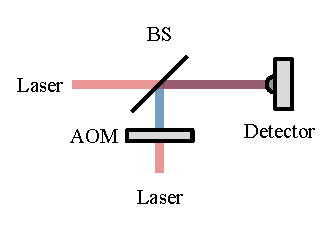
\includegraphics{part1/Figs/HeterodyneTwoLasers.pdf}
    \end{subfigure}
    \begin{subfigure}{0.49\linewidth}
    %\centering
    %% Creator: Matplotlib, PGF backend
%%
%% To include the figure in your LaTeX document, write
%%   \input{<filename>.pgf}
%%
%% Make sure the required packages are loaded in your preamble
%%   \usepackage{pgf}
%%
%% Figures using additional raster images can only be included by \input if
%% they are in the same directory as the main LaTeX file. For loading figures
%% from other directories you can use the `import` package
%%   \usepackage{import}
%% and then include the figures with
%%   \import{<path to file>}{<filename>.pgf}
%%
%% Matplotlib used the following preamble
%%
\begingroup%
\makeatletter%
\begin{pgfpicture}%
\pgfpathrectangle{\pgfpointorigin}{\pgfqpoint{2.855000in}{1.427500in}}%
\pgfusepath{use as bounding box, clip}%
\begin{pgfscope}%
\pgfsetbuttcap%
\pgfsetmiterjoin%
\definecolor{currentfill}{rgb}{1.000000,1.000000,1.000000}%
\pgfsetfillcolor{currentfill}%
\pgfsetlinewidth{0.000000pt}%
\definecolor{currentstroke}{rgb}{1.000000,1.000000,1.000000}%
\pgfsetstrokecolor{currentstroke}%
\pgfsetdash{}{0pt}%
\pgfpathmoveto{\pgfqpoint{0.000000in}{0.000000in}}%
\pgfpathlineto{\pgfqpoint{2.855000in}{0.000000in}}%
\pgfpathlineto{\pgfqpoint{2.855000in}{1.427500in}}%
\pgfpathlineto{\pgfqpoint{0.000000in}{1.427500in}}%
\pgfpathclose%
\pgfusepath{fill}%
\end{pgfscope}%
\begin{pgfscope}%
\pgfsetbuttcap%
\pgfsetmiterjoin%
\definecolor{currentfill}{rgb}{1.000000,1.000000,1.000000}%
\pgfsetfillcolor{currentfill}%
\pgfsetlinewidth{0.000000pt}%
\definecolor{currentstroke}{rgb}{0.000000,0.000000,0.000000}%
\pgfsetstrokecolor{currentstroke}%
\pgfsetstrokeopacity{0.000000}%
\pgfsetdash{}{0pt}%
\pgfpathmoveto{\pgfqpoint{0.342732in}{0.521851in}}%
\pgfpathlineto{\pgfqpoint{1.130154in}{0.521851in}}%
\pgfpathlineto{\pgfqpoint{1.130154in}{1.277500in}}%
\pgfpathlineto{\pgfqpoint{0.342732in}{1.277500in}}%
\pgfpathclose%
\pgfusepath{fill}%
\end{pgfscope}%
\begin{pgfscope}%
\pgfpathrectangle{\pgfqpoint{0.342732in}{0.521851in}}{\pgfqpoint{0.787423in}{0.755649in}} %
\pgfusepath{clip}%
\pgfsetrectcap%
\pgfsetroundjoin%
\pgfsetlinewidth{1.003750pt}%
\definecolor{currentstroke}{rgb}{0.600000,0.000000,0.000000}%
\pgfsetstrokecolor{currentstroke}%
\pgfsetdash{}{0pt}%
\pgfpathmoveto{\pgfqpoint{0.342732in}{0.521851in}}%
\pgfpathlineto{\pgfqpoint{0.570525in}{0.522959in}}%
\pgfpathlineto{\pgfqpoint{0.586289in}{0.525344in}}%
\pgfpathlineto{\pgfqpoint{0.597324in}{0.529138in}}%
\pgfpathlineto{\pgfqpoint{0.605994in}{0.534336in}}%
\pgfpathlineto{\pgfqpoint{0.613876in}{0.541618in}}%
\pgfpathlineto{\pgfqpoint{0.621758in}{0.552265in}}%
\pgfpathlineto{\pgfqpoint{0.628852in}{0.565587in}}%
\pgfpathlineto{\pgfqpoint{0.636734in}{0.585580in}}%
\pgfpathlineto{\pgfqpoint{0.644617in}{0.612092in}}%
\pgfpathlineto{\pgfqpoint{0.653287in}{0.649852in}}%
\pgfpathlineto{\pgfqpoint{0.662745in}{0.702014in}}%
\pgfpathlineto{\pgfqpoint{0.673780in}{0.776670in}}%
\pgfpathlineto{\pgfqpoint{0.689545in}{0.901214in}}%
\pgfpathlineto{\pgfqpoint{0.708462in}{1.047619in}}%
\pgfpathlineto{\pgfqpoint{0.717920in}{1.103696in}}%
\pgfpathlineto{\pgfqpoint{0.725014in}{1.132889in}}%
\pgfpathlineto{\pgfqpoint{0.730532in}{1.146509in}}%
\pgfpathlineto{\pgfqpoint{0.734473in}{1.150995in}}%
\pgfpathlineto{\pgfqpoint{0.737625in}{1.151356in}}%
\pgfpathlineto{\pgfqpoint{0.740778in}{1.148838in}}%
\pgfpathlineto{\pgfqpoint{0.744719in}{1.141699in}}%
\pgfpathlineto{\pgfqpoint{0.749449in}{1.127490in}}%
\pgfpathlineto{\pgfqpoint{0.755754in}{1.099712in}}%
\pgfpathlineto{\pgfqpoint{0.763636in}{1.052913in}}%
\pgfpathlineto{\pgfqpoint{0.774671in}{0.971536in}}%
\pgfpathlineto{\pgfqpoint{0.807776in}{0.716827in}}%
\pgfpathlineto{\pgfqpoint{0.818811in}{0.653758in}}%
\pgfpathlineto{\pgfqpoint{0.828270in}{0.612092in}}%
\pgfpathlineto{\pgfqpoint{0.836940in}{0.583305in}}%
\pgfpathlineto{\pgfqpoint{0.845610in}{0.562276in}}%
\pgfpathlineto{\pgfqpoint{0.853492in}{0.548657in}}%
\pgfpathlineto{\pgfqpoint{0.861375in}{0.539125in}}%
\pgfpathlineto{\pgfqpoint{0.870045in}{0.532157in}}%
\pgfpathlineto{\pgfqpoint{0.879503in}{0.527491in}}%
\pgfpathlineto{\pgfqpoint{0.891327in}{0.524356in}}%
\pgfpathlineto{\pgfqpoint{0.907879in}{0.522573in}}%
\pgfpathlineto{\pgfqpoint{0.940196in}{0.521896in}}%
\pgfpathlineto{\pgfqpoint{1.130154in}{0.521851in}}%
\pgfpathlineto{\pgfqpoint{1.130154in}{0.521851in}}%
\pgfusepath{stroke}%
\end{pgfscope}%
\begin{pgfscope}%
\pgfsetrectcap%
\pgfsetmiterjoin%
\pgfsetlinewidth{1.003750pt}%
\definecolor{currentstroke}{rgb}{0.000000,0.000000,0.000000}%
\pgfsetstrokecolor{currentstroke}%
\pgfsetdash{}{0pt}%
\pgfpathmoveto{\pgfqpoint{0.342732in}{1.277500in}}%
\pgfpathlineto{\pgfqpoint{1.130154in}{1.277500in}}%
\pgfusepath{stroke}%
\end{pgfscope}%
\begin{pgfscope}%
\pgfsetrectcap%
\pgfsetmiterjoin%
\pgfsetlinewidth{1.003750pt}%
\definecolor{currentstroke}{rgb}{0.000000,0.000000,0.000000}%
\pgfsetstrokecolor{currentstroke}%
\pgfsetdash{}{0pt}%
\pgfpathmoveto{\pgfqpoint{0.342732in}{0.521851in}}%
\pgfpathlineto{\pgfqpoint{0.342732in}{1.277500in}}%
\pgfusepath{stroke}%
\end{pgfscope}%
\begin{pgfscope}%
\pgfsetrectcap%
\pgfsetmiterjoin%
\pgfsetlinewidth{1.003750pt}%
\definecolor{currentstroke}{rgb}{0.000000,0.000000,0.000000}%
\pgfsetstrokecolor{currentstroke}%
\pgfsetdash{}{0pt}%
\pgfpathmoveto{\pgfqpoint{1.130154in}{0.521851in}}%
\pgfpathlineto{\pgfqpoint{1.130154in}{1.277500in}}%
\pgfusepath{stroke}%
\end{pgfscope}%
\begin{pgfscope}%
\pgfsetrectcap%
\pgfsetmiterjoin%
\pgfsetlinewidth{1.003750pt}%
\definecolor{currentstroke}{rgb}{0.000000,0.000000,0.000000}%
\pgfsetstrokecolor{currentstroke}%
\pgfsetdash{}{0pt}%
\pgfpathmoveto{\pgfqpoint{0.342732in}{0.521851in}}%
\pgfpathlineto{\pgfqpoint{1.130154in}{0.521851in}}%
\pgfusepath{stroke}%
\end{pgfscope}%
\begin{pgfscope}%
\pgfsetbuttcap%
\pgfsetroundjoin%
\definecolor{currentfill}{rgb}{0.000000,0.000000,0.000000}%
\pgfsetfillcolor{currentfill}%
\pgfsetlinewidth{0.501875pt}%
\definecolor{currentstroke}{rgb}{0.000000,0.000000,0.000000}%
\pgfsetstrokecolor{currentstroke}%
\pgfsetdash{}{0pt}%
\pgfsys@defobject{currentmarker}{\pgfqpoint{0.000000in}{0.000000in}}{\pgfqpoint{0.000000in}{0.055556in}}{%
\pgfpathmoveto{\pgfqpoint{0.000000in}{0.000000in}}%
\pgfpathlineto{\pgfqpoint{0.000000in}{0.055556in}}%
\pgfusepath{stroke,fill}%
}%
\begin{pgfscope}%
\pgfsys@transformshift{0.736443in}{0.521851in}%
\pgfsys@useobject{currentmarker}{}%
\end{pgfscope}%
\end{pgfscope}%
\begin{pgfscope}%
\pgfsetbuttcap%
\pgfsetroundjoin%
\definecolor{currentfill}{rgb}{0.000000,0.000000,0.000000}%
\pgfsetfillcolor{currentfill}%
\pgfsetlinewidth{0.501875pt}%
\definecolor{currentstroke}{rgb}{0.000000,0.000000,0.000000}%
\pgfsetstrokecolor{currentstroke}%
\pgfsetdash{}{0pt}%
\pgfsys@defobject{currentmarker}{\pgfqpoint{0.000000in}{-0.055556in}}{\pgfqpoint{0.000000in}{0.000000in}}{%
\pgfpathmoveto{\pgfqpoint{0.000000in}{0.000000in}}%
\pgfpathlineto{\pgfqpoint{0.000000in}{-0.055556in}}%
\pgfusepath{stroke,fill}%
}%
\begin{pgfscope}%
\pgfsys@transformshift{0.736443in}{1.277500in}%
\pgfsys@useobject{currentmarker}{}%
\end{pgfscope}%
\end{pgfscope}%
\begin{pgfscope}%
\pgftext[x=0.736443in,y=0.466296in,,top]{\fontsize{10.000000}{12.000000}\selectfont \(\displaystyle \omega_1\)}%
\end{pgfscope}%
\begin{pgfscope}%
\pgftext[x=0.273287in,y=0.899676in,,bottom,rotate=90.000000]{\fontsize{10.000000}{12.000000}\selectfont Amplitude}%
\end{pgfscope}%
\begin{pgfscope}%
\pgfsetbuttcap%
\pgfsetmiterjoin%
\definecolor{currentfill}{rgb}{1.000000,1.000000,1.000000}%
\pgfsetfillcolor{currentfill}%
\pgfsetlinewidth{0.000000pt}%
\definecolor{currentstroke}{rgb}{0.000000,0.000000,0.000000}%
\pgfsetstrokecolor{currentstroke}%
\pgfsetstrokeopacity{0.000000}%
\pgfsetdash{}{0pt}%
\pgfpathmoveto{\pgfqpoint{1.130154in}{0.521851in}}%
\pgfpathlineto{\pgfqpoint{1.917577in}{0.521851in}}%
\pgfpathlineto{\pgfqpoint{1.917577in}{1.277500in}}%
\pgfpathlineto{\pgfqpoint{1.130154in}{1.277500in}}%
\pgfpathclose%
\pgfusepath{fill}%
\end{pgfscope}%
\begin{pgfscope}%
\pgfpathrectangle{\pgfqpoint{1.130154in}{0.521851in}}{\pgfqpoint{0.787423in}{0.755649in}} %
\pgfusepath{clip}%
\pgfsetrectcap%
\pgfsetroundjoin%
\pgfsetlinewidth{1.003750pt}%
\definecolor{currentstroke}{rgb}{0.043137,0.325490,0.580392}%
\pgfsetstrokecolor{currentstroke}%
\pgfsetdash{}{0pt}%
\pgfpathmoveto{\pgfqpoint{1.130154in}{0.521851in}}%
\pgfpathlineto{\pgfqpoint{1.346124in}{0.522931in}}%
\pgfpathlineto{\pgfqpoint{1.363465in}{0.525371in}}%
\pgfpathlineto{\pgfqpoint{1.375288in}{0.529202in}}%
\pgfpathlineto{\pgfqpoint{1.384747in}{0.534575in}}%
\pgfpathlineto{\pgfqpoint{1.393417in}{0.542233in}}%
\pgfpathlineto{\pgfqpoint{1.401299in}{0.552319in}}%
\pgfpathlineto{\pgfqpoint{1.409181in}{0.566271in}}%
\pgfpathlineto{\pgfqpoint{1.417063in}{0.585009in}}%
\pgfpathlineto{\pgfqpoint{1.424945in}{0.609429in}}%
\pgfpathlineto{\pgfqpoint{1.433616in}{0.643750in}}%
\pgfpathlineto{\pgfqpoint{1.443074in}{0.690758in}}%
\pgfpathlineto{\pgfqpoint{1.454109in}{0.757953in}}%
\pgfpathlineto{\pgfqpoint{1.468297in}{0.859744in}}%
\pgfpathlineto{\pgfqpoint{1.495096in}{1.054781in}}%
\pgfpathlineto{\pgfqpoint{1.504555in}{1.105952in}}%
\pgfpathlineto{\pgfqpoint{1.511649in}{1.132892in}}%
\pgfpathlineto{\pgfqpoint{1.517166in}{1.145886in}}%
\pgfpathlineto{\pgfqpoint{1.521107in}{1.150593in}}%
\pgfpathlineto{\pgfqpoint{1.524260in}{1.151539in}}%
\pgfpathlineto{\pgfqpoint{1.527413in}{1.149963in}}%
\pgfpathlineto{\pgfqpoint{1.531354in}{1.144481in}}%
\pgfpathlineto{\pgfqpoint{1.536083in}{1.132892in}}%
\pgfpathlineto{\pgfqpoint{1.541601in}{1.112870in}}%
\pgfpathlineto{\pgfqpoint{1.548695in}{1.077966in}}%
\pgfpathlineto{\pgfqpoint{1.558153in}{1.018682in}}%
\pgfpathlineto{\pgfqpoint{1.573129in}{0.907912in}}%
\pgfpathlineto{\pgfqpoint{1.594411in}{0.752748in}}%
\pgfpathlineto{\pgfqpoint{1.606234in}{0.682222in}}%
\pgfpathlineto{\pgfqpoint{1.616481in}{0.633574in}}%
\pgfpathlineto{\pgfqpoint{1.625939in}{0.598926in}}%
\pgfpathlineto{\pgfqpoint{1.634610in}{0.574983in}}%
\pgfpathlineto{\pgfqpoint{1.643280in}{0.557385in}}%
\pgfpathlineto{\pgfqpoint{1.651950in}{0.544906in}}%
\pgfpathlineto{\pgfqpoint{1.660620in}{0.536363in}}%
\pgfpathlineto{\pgfqpoint{1.670079in}{0.530311in}}%
\pgfpathlineto{\pgfqpoint{1.680326in}{0.526379in}}%
\pgfpathlineto{\pgfqpoint{1.693725in}{0.523726in}}%
\pgfpathlineto{\pgfqpoint{1.714219in}{0.522275in}}%
\pgfpathlineto{\pgfqpoint{1.762300in}{0.521858in}}%
\pgfpathlineto{\pgfqpoint{1.917577in}{0.521851in}}%
\pgfpathlineto{\pgfqpoint{1.917577in}{0.521851in}}%
\pgfusepath{stroke}%
\end{pgfscope}%
\begin{pgfscope}%
\pgfsetrectcap%
\pgfsetmiterjoin%
\pgfsetlinewidth{1.003750pt}%
\definecolor{currentstroke}{rgb}{0.000000,0.000000,0.000000}%
\pgfsetstrokecolor{currentstroke}%
\pgfsetdash{}{0pt}%
\pgfpathmoveto{\pgfqpoint{1.130154in}{1.277500in}}%
\pgfpathlineto{\pgfqpoint{1.917577in}{1.277500in}}%
\pgfusepath{stroke}%
\end{pgfscope}%
\begin{pgfscope}%
\pgfsetrectcap%
\pgfsetmiterjoin%
\pgfsetlinewidth{1.003750pt}%
\definecolor{currentstroke}{rgb}{0.000000,0.000000,0.000000}%
\pgfsetstrokecolor{currentstroke}%
\pgfsetdash{}{0pt}%
\pgfpathmoveto{\pgfqpoint{1.130154in}{0.521851in}}%
\pgfpathlineto{\pgfqpoint{1.130154in}{1.277500in}}%
\pgfusepath{stroke}%
\end{pgfscope}%
\begin{pgfscope}%
\pgfsetrectcap%
\pgfsetmiterjoin%
\pgfsetlinewidth{1.003750pt}%
\definecolor{currentstroke}{rgb}{0.000000,0.000000,0.000000}%
\pgfsetstrokecolor{currentstroke}%
\pgfsetdash{}{0pt}%
\pgfpathmoveto{\pgfqpoint{1.917577in}{0.521851in}}%
\pgfpathlineto{\pgfqpoint{1.917577in}{1.277500in}}%
\pgfusepath{stroke}%
\end{pgfscope}%
\begin{pgfscope}%
\pgfsetrectcap%
\pgfsetmiterjoin%
\pgfsetlinewidth{1.003750pt}%
\definecolor{currentstroke}{rgb}{0.000000,0.000000,0.000000}%
\pgfsetstrokecolor{currentstroke}%
\pgfsetdash{}{0pt}%
\pgfpathmoveto{\pgfqpoint{1.130154in}{0.521851in}}%
\pgfpathlineto{\pgfqpoint{1.917577in}{0.521851in}}%
\pgfusepath{stroke}%
\end{pgfscope}%
\begin{pgfscope}%
\pgfsetbuttcap%
\pgfsetroundjoin%
\definecolor{currentfill}{rgb}{0.000000,0.000000,0.000000}%
\pgfsetfillcolor{currentfill}%
\pgfsetlinewidth{0.501875pt}%
\definecolor{currentstroke}{rgb}{0.000000,0.000000,0.000000}%
\pgfsetstrokecolor{currentstroke}%
\pgfsetdash{}{0pt}%
\pgfsys@defobject{currentmarker}{\pgfqpoint{0.000000in}{0.000000in}}{\pgfqpoint{0.000000in}{0.055556in}}{%
\pgfpathmoveto{\pgfqpoint{0.000000in}{0.000000in}}%
\pgfpathlineto{\pgfqpoint{0.000000in}{0.055556in}}%
\pgfusepath{stroke,fill}%
}%
\begin{pgfscope}%
\pgfsys@transformshift{1.523866in}{0.521851in}%
\pgfsys@useobject{currentmarker}{}%
\end{pgfscope}%
\end{pgfscope}%
\begin{pgfscope}%
\pgfsetbuttcap%
\pgfsetroundjoin%
\definecolor{currentfill}{rgb}{0.000000,0.000000,0.000000}%
\pgfsetfillcolor{currentfill}%
\pgfsetlinewidth{0.501875pt}%
\definecolor{currentstroke}{rgb}{0.000000,0.000000,0.000000}%
\pgfsetstrokecolor{currentstroke}%
\pgfsetdash{}{0pt}%
\pgfsys@defobject{currentmarker}{\pgfqpoint{0.000000in}{-0.055556in}}{\pgfqpoint{0.000000in}{0.000000in}}{%
\pgfpathmoveto{\pgfqpoint{0.000000in}{0.000000in}}%
\pgfpathlineto{\pgfqpoint{0.000000in}{-0.055556in}}%
\pgfusepath{stroke,fill}%
}%
\begin{pgfscope}%
\pgfsys@transformshift{1.523866in}{1.277500in}%
\pgfsys@useobject{currentmarker}{}%
\end{pgfscope}%
\end{pgfscope}%
\begin{pgfscope}%
\pgftext[x=1.523866in,y=0.466296in,,top]{\fontsize{10.000000}{12.000000}\selectfont \(\displaystyle \omega_1+\delta\)}%
\end{pgfscope}%
\begin{pgfscope}%
\pgftext[x=1.523866in,y=0.273395in,,top]{\fontsize{10.000000}{12.000000}\selectfont Frequency}%
\end{pgfscope}%
\begin{pgfscope}%
\pgfsetbuttcap%
\pgfsetmiterjoin%
\definecolor{currentfill}{rgb}{1.000000,1.000000,1.000000}%
\pgfsetfillcolor{currentfill}%
\pgfsetlinewidth{0.000000pt}%
\definecolor{currentstroke}{rgb}{0.000000,0.000000,0.000000}%
\pgfsetstrokecolor{currentstroke}%
\pgfsetstrokeopacity{0.000000}%
\pgfsetdash{}{0pt}%
\pgfpathmoveto{\pgfqpoint{1.917577in}{0.521851in}}%
\pgfpathlineto{\pgfqpoint{2.705000in}{0.521851in}}%
\pgfpathlineto{\pgfqpoint{2.705000in}{1.277500in}}%
\pgfpathlineto{\pgfqpoint{1.917577in}{1.277500in}}%
\pgfpathclose%
\pgfusepath{fill}%
\end{pgfscope}%
\begin{pgfscope}%
\pgfpathrectangle{\pgfqpoint{1.917577in}{0.521851in}}{\pgfqpoint{0.787423in}{0.755649in}} %
\pgfusepath{clip}%
\pgfsetrectcap%
\pgfsetroundjoin%
\pgfsetlinewidth{1.003750pt}%
\definecolor{currentstroke}{rgb}{0.301961,0.607843,0.301961}%
\pgfsetstrokecolor{currentstroke}%
\pgfsetdash{}{0pt}%
\pgfpathmoveto{\pgfqpoint{1.917577in}{0.521851in}}%
\pgfpathlineto{\pgfqpoint{2.068126in}{0.522921in}}%
\pgfpathlineto{\pgfqpoint{2.091772in}{0.525326in}}%
\pgfpathlineto{\pgfqpoint{2.107536in}{0.528981in}}%
\pgfpathlineto{\pgfqpoint{2.120147in}{0.534043in}}%
\pgfpathlineto{\pgfqpoint{2.131182in}{0.540809in}}%
\pgfpathlineto{\pgfqpoint{2.141429in}{0.549751in}}%
\pgfpathlineto{\pgfqpoint{2.150888in}{0.560919in}}%
\pgfpathlineto{\pgfqpoint{2.160346in}{0.575515in}}%
\pgfpathlineto{\pgfqpoint{2.169805in}{0.594159in}}%
\pgfpathlineto{\pgfqpoint{2.180051in}{0.619587in}}%
\pgfpathlineto{\pgfqpoint{2.190298in}{0.651007in}}%
\pgfpathlineto{\pgfqpoint{2.202121in}{0.695079in}}%
\pgfpathlineto{\pgfqpoint{2.214733in}{0.751060in}}%
\pgfpathlineto{\pgfqpoint{2.230497in}{0.831851in}}%
\pgfpathlineto{\pgfqpoint{2.274637in}{1.065169in}}%
\pgfpathlineto{\pgfqpoint{2.284884in}{1.104762in}}%
\pgfpathlineto{\pgfqpoint{2.293554in}{1.129695in}}%
\pgfpathlineto{\pgfqpoint{2.300648in}{1.143368in}}%
\pgfpathlineto{\pgfqpoint{2.306165in}{1.149501in}}%
\pgfpathlineto{\pgfqpoint{2.310895in}{1.151517in}}%
\pgfpathlineto{\pgfqpoint{2.314836in}{1.150886in}}%
\pgfpathlineto{\pgfqpoint{2.318777in}{1.148161in}}%
\pgfpathlineto{\pgfqpoint{2.323506in}{1.142165in}}%
\pgfpathlineto{\pgfqpoint{2.329023in}{1.131525in}}%
\pgfpathlineto{\pgfqpoint{2.336117in}{1.112405in}}%
\pgfpathlineto{\pgfqpoint{2.344788in}{1.081562in}}%
\pgfpathlineto{\pgfqpoint{2.355034in}{1.036346in}}%
\pgfpathlineto{\pgfqpoint{2.369222in}{0.962954in}}%
\pgfpathlineto{\pgfqpoint{2.411786in}{0.736249in}}%
\pgfpathlineto{\pgfqpoint{2.425185in}{0.679455in}}%
\pgfpathlineto{\pgfqpoint{2.437008in}{0.638187in}}%
\pgfpathlineto{\pgfqpoint{2.448043in}{0.607136in}}%
\pgfpathlineto{\pgfqpoint{2.458290in}{0.584293in}}%
\pgfpathlineto{\pgfqpoint{2.468537in}{0.566548in}}%
\pgfpathlineto{\pgfqpoint{2.478783in}{0.553132in}}%
\pgfpathlineto{\pgfqpoint{2.489030in}{0.543254in}}%
\pgfpathlineto{\pgfqpoint{2.500065in}{0.535719in}}%
\pgfpathlineto{\pgfqpoint{2.511888in}{0.530313in}}%
\pgfpathlineto{\pgfqpoint{2.526076in}{0.526347in}}%
\pgfpathlineto{\pgfqpoint{2.544205in}{0.523733in}}%
\pgfpathlineto{\pgfqpoint{2.571792in}{0.522288in}}%
\pgfpathlineto{\pgfqpoint{2.635637in}{0.521859in}}%
\pgfpathlineto{\pgfqpoint{2.705000in}{0.521851in}}%
\pgfpathlineto{\pgfqpoint{2.705000in}{0.521851in}}%
\pgfusepath{stroke}%
\end{pgfscope}%
\begin{pgfscope}%
\pgfpathrectangle{\pgfqpoint{1.917577in}{0.521851in}}{\pgfqpoint{0.787423in}{0.755649in}} %
\pgfusepath{clip}%
\pgfsetbuttcap%
\pgfsetroundjoin%
\pgfsetlinewidth{1.003750pt}%
\definecolor{currentstroke}{rgb}{0.600000,0.000000,0.000000}%
\pgfsetstrokecolor{currentstroke}%
\pgfsetdash{{1.000000pt}{3.000000pt}}{0.000000pt}%
\pgfpathmoveto{\pgfqpoint{1.917577in}{0.521851in}}%
\pgfpathlineto{\pgfqpoint{2.145370in}{0.522959in}}%
\pgfpathlineto{\pgfqpoint{2.161134in}{0.525344in}}%
\pgfpathlineto{\pgfqpoint{2.172169in}{0.529138in}}%
\pgfpathlineto{\pgfqpoint{2.180840in}{0.534336in}}%
\pgfpathlineto{\pgfqpoint{2.188722in}{0.541618in}}%
\pgfpathlineto{\pgfqpoint{2.196604in}{0.552265in}}%
\pgfpathlineto{\pgfqpoint{2.203698in}{0.565587in}}%
\pgfpathlineto{\pgfqpoint{2.211580in}{0.585580in}}%
\pgfpathlineto{\pgfqpoint{2.219462in}{0.612092in}}%
\pgfpathlineto{\pgfqpoint{2.228132in}{0.649852in}}%
\pgfpathlineto{\pgfqpoint{2.237591in}{0.702014in}}%
\pgfpathlineto{\pgfqpoint{2.248626in}{0.776670in}}%
\pgfpathlineto{\pgfqpoint{2.264390in}{0.901214in}}%
\pgfpathlineto{\pgfqpoint{2.283307in}{1.047619in}}%
\pgfpathlineto{\pgfqpoint{2.292766in}{1.103696in}}%
\pgfpathlineto{\pgfqpoint{2.299860in}{1.132889in}}%
\pgfpathlineto{\pgfqpoint{2.305377in}{1.146509in}}%
\pgfpathlineto{\pgfqpoint{2.309318in}{1.150995in}}%
\pgfpathlineto{\pgfqpoint{2.312471in}{1.151356in}}%
\pgfpathlineto{\pgfqpoint{2.315624in}{1.148838in}}%
\pgfpathlineto{\pgfqpoint{2.319565in}{1.141699in}}%
\pgfpathlineto{\pgfqpoint{2.324294in}{1.127490in}}%
\pgfpathlineto{\pgfqpoint{2.330600in}{1.099712in}}%
\pgfpathlineto{\pgfqpoint{2.338482in}{1.052913in}}%
\pgfpathlineto{\pgfqpoint{2.349517in}{0.971536in}}%
\pgfpathlineto{\pgfqpoint{2.382622in}{0.716827in}}%
\pgfpathlineto{\pgfqpoint{2.393657in}{0.653758in}}%
\pgfpathlineto{\pgfqpoint{2.403115in}{0.612092in}}%
\pgfpathlineto{\pgfqpoint{2.411786in}{0.583305in}}%
\pgfpathlineto{\pgfqpoint{2.420456in}{0.562276in}}%
\pgfpathlineto{\pgfqpoint{2.428338in}{0.548657in}}%
\pgfpathlineto{\pgfqpoint{2.436220in}{0.539125in}}%
\pgfpathlineto{\pgfqpoint{2.444890in}{0.532157in}}%
\pgfpathlineto{\pgfqpoint{2.454349in}{0.527491in}}%
\pgfpathlineto{\pgfqpoint{2.466172in}{0.524356in}}%
\pgfpathlineto{\pgfqpoint{2.482725in}{0.522573in}}%
\pgfpathlineto{\pgfqpoint{2.515041in}{0.521896in}}%
\pgfpathlineto{\pgfqpoint{2.705000in}{0.521851in}}%
\pgfpathlineto{\pgfqpoint{2.705000in}{0.521851in}}%
\pgfusepath{stroke}%
\end{pgfscope}%
\begin{pgfscope}%
\pgfsetrectcap%
\pgfsetmiterjoin%
\pgfsetlinewidth{1.003750pt}%
\definecolor{currentstroke}{rgb}{0.000000,0.000000,0.000000}%
\pgfsetstrokecolor{currentstroke}%
\pgfsetdash{}{0pt}%
\pgfpathmoveto{\pgfqpoint{1.917577in}{1.277500in}}%
\pgfpathlineto{\pgfqpoint{2.705000in}{1.277500in}}%
\pgfusepath{stroke}%
\end{pgfscope}%
\begin{pgfscope}%
\pgfsetrectcap%
\pgfsetmiterjoin%
\pgfsetlinewidth{1.003750pt}%
\definecolor{currentstroke}{rgb}{0.000000,0.000000,0.000000}%
\pgfsetstrokecolor{currentstroke}%
\pgfsetdash{}{0pt}%
\pgfpathmoveto{\pgfqpoint{1.917577in}{0.521851in}}%
\pgfpathlineto{\pgfqpoint{1.917577in}{1.277500in}}%
\pgfusepath{stroke}%
\end{pgfscope}%
\begin{pgfscope}%
\pgfsetrectcap%
\pgfsetmiterjoin%
\pgfsetlinewidth{1.003750pt}%
\definecolor{currentstroke}{rgb}{0.000000,0.000000,0.000000}%
\pgfsetstrokecolor{currentstroke}%
\pgfsetdash{}{0pt}%
\pgfpathmoveto{\pgfqpoint{2.705000in}{0.521851in}}%
\pgfpathlineto{\pgfqpoint{2.705000in}{1.277500in}}%
\pgfusepath{stroke}%
\end{pgfscope}%
\begin{pgfscope}%
\pgfsetrectcap%
\pgfsetmiterjoin%
\pgfsetlinewidth{1.003750pt}%
\definecolor{currentstroke}{rgb}{0.000000,0.000000,0.000000}%
\pgfsetstrokecolor{currentstroke}%
\pgfsetdash{}{0pt}%
\pgfpathmoveto{\pgfqpoint{1.917577in}{0.521851in}}%
\pgfpathlineto{\pgfqpoint{2.705000in}{0.521851in}}%
\pgfusepath{stroke}%
\end{pgfscope}%
\begin{pgfscope}%
\pgfsetbuttcap%
\pgfsetroundjoin%
\definecolor{currentfill}{rgb}{0.000000,0.000000,0.000000}%
\pgfsetfillcolor{currentfill}%
\pgfsetlinewidth{0.501875pt}%
\definecolor{currentstroke}{rgb}{0.000000,0.000000,0.000000}%
\pgfsetstrokecolor{currentstroke}%
\pgfsetdash{}{0pt}%
\pgfsys@defobject{currentmarker}{\pgfqpoint{0.000000in}{0.000000in}}{\pgfqpoint{0.000000in}{0.055556in}}{%
\pgfpathmoveto{\pgfqpoint{0.000000in}{0.000000in}}%
\pgfpathlineto{\pgfqpoint{0.000000in}{0.055556in}}%
\pgfusepath{stroke,fill}%
}%
\begin{pgfscope}%
\pgfsys@transformshift{2.311289in}{0.521851in}%
\pgfsys@useobject{currentmarker}{}%
\end{pgfscope}%
\end{pgfscope}%
\begin{pgfscope}%
\pgfsetbuttcap%
\pgfsetroundjoin%
\definecolor{currentfill}{rgb}{0.000000,0.000000,0.000000}%
\pgfsetfillcolor{currentfill}%
\pgfsetlinewidth{0.501875pt}%
\definecolor{currentstroke}{rgb}{0.000000,0.000000,0.000000}%
\pgfsetstrokecolor{currentstroke}%
\pgfsetdash{}{0pt}%
\pgfsys@defobject{currentmarker}{\pgfqpoint{0.000000in}{-0.055556in}}{\pgfqpoint{0.000000in}{0.000000in}}{%
\pgfpathmoveto{\pgfqpoint{0.000000in}{0.000000in}}%
\pgfpathlineto{\pgfqpoint{0.000000in}{-0.055556in}}%
\pgfusepath{stroke,fill}%
}%
\begin{pgfscope}%
\pgfsys@transformshift{2.311289in}{1.277500in}%
\pgfsys@useobject{currentmarker}{}%
\end{pgfscope}%
\end{pgfscope}%
\begin{pgfscope}%
\pgftext[x=2.311289in,y=0.466296in,,top]{\fontsize{10.000000}{12.000000}\selectfont \(\displaystyle \delta\)}%
\end{pgfscope}%
\end{pgfpicture}%
\makeatother%
\endgroup%

    \end{subfigure}
    \caption{Heterodyne measurement with two `identical' lasers. One beam is frequency shifted by an \gls{aom} from the initial frequency ($\omega_1$, red) to an offset frequency ($\omega_1+\delta$, blue) to enable measurement by a spectrum analyser. Shown on the right is the spectral lineshapes of the lasers and the heterodyne beatnote (green).}
\end{figure}

\subsubsection{Linewidth Discrepancies}
{\color{red}I'm not certain enough about what's going on here so just remove this.}

There is an interesting discrepancy between intuition and what the literature uses to describe `linewidth'.
Intuitively, when discussing the spectral properties of light, one would expect references to refer to the properties of the electric field since that is the entity that is interacting with atoms and other frequency references.
However, the literature seems to exclusively refer to properties of the power of the signal from photodetectors, as shown on spectrum analysers, which differ by a factor of 2 which will be shown below.
Despite this fact this document follows the convention to avoid confusion.

The simplest way to examine a heterodyne signal is to look at the signal from the detector on a radio-frequency spectrum analyser.
A spectrum analyser shows the power for each frequency component of the input electrical signal.
The power of the electrical signal from the detector, $P_{elec}$ is roughly:
\begin{equation}
P_{elec}\propto I^2 \propto E^2
\label{eq:beatnote_proportional}
\end{equation}
where $I$ is the light intensity incident on the detector and $E$ is the electric field incident on the detector.

Of primary interest are the spectral properties of these signals which are given by their Fourier transform.
However we cannot simply write
\begin{equation}
\mathcal{F}[P_{elec}]\propto \mathcal{F}[I^2] \propto \mathcal{F}[E^2]
\end{equation}
since it's not true.
The inverse convolution theorem, however, can be used
\begin{equation}
f\cdot g = \mathcal{F}^{-1} \bigg[ \mathcal{F}[f] \otimes\mathcal{F}[g]\bigg].
\end{equation}

So Equation~\ref{eq:beatnote_proportional} in Fourier space becomes
\begin{align}
\mathcal{F}[P_{elec}]&\propto \mathcal{F}[I]\otimes\mathcal{F}[I]\nonumber\\
&\propto \big\{\mathcal{F}[E] \otimes\mathcal{F}[E]\big\} \otimes\big\{\mathcal{F}[E] \otimes\mathcal{F}[E]\big\}
\end{align}

For a Gaussian lineshape beatnote with \gls{rms} width $\sigma$, we can write
\begin{equation}
\mathcal{F}[E] = A e^{-(f-f_0)^2/2\sigma^2}.
\end{equation}

It is easy to show that the convolution of two Gaussians produces another Gaussian with variance equal to the sum of the variance of the two constituent functions.
Thus,
\begin{equation}
\mathcal{F}[I] = B e^{-(f-f_0)^2/4\sigma^2}
\end{equation}
and
\begin{align}
\mathcal{F}[P] &= B e^{-(f-f_0)^2/8\sigma^2}\nonumber\\
&= B e^{-(f-f_0)^2/2(2\sigma)^2}
\end{align}
So the width of the signal shown on a spectrum analyser has twice the spectral width of the electric field that generated it.

\subsection{cavity Measurements}

\subsubsection{Two-Sided Peak Measurements}

\subsubsection{One_Sided Peak Measurements}

\subsection{Noise measurements}

\subsubsection{Bandwidth Stuff}

\subsubsection{Noise Integration}

\subsection{Long Term Stability}

